\documentclass[11pt]{article}

    \usepackage[breakable]{tcolorbox}
    \usepackage{parskip} % Stop auto-indenting (to mimic markdown behaviour)
    

    % Basic figure setup, for now with no caption control since it's done
    % automatically by Pandoc (which extracts ![](path) syntax from Markdown).
    \usepackage{graphicx}
    % Maintain compatibility with old templates. Remove in nbconvert 6.0
    \let\Oldincludegraphics\includegraphics
    % Ensure that by default, figures have no caption (until we provide a
    % proper Figure object with a Caption API and a way to capture that
    % in the conversion process - todo).
    \usepackage{caption}
    \DeclareCaptionFormat{nocaption}{}
    \captionsetup{format=nocaption,aboveskip=0pt,belowskip=0pt}

    \usepackage{float}
    \floatplacement{figure}{H} % forces figures to be placed at the correct location
    \usepackage{xcolor} % Allow colors to be defined
    \usepackage{enumerate} % Needed for markdown enumerations to work
    \usepackage{geometry} % Used to adjust the document margins
    \usepackage{amsmath} % Equations
    \usepackage{amssymb} % Equations
    \usepackage{textcomp} % defines textquotesingle
    % Hack from http://tex.stackexchange.com/a/47451/13684:
    \AtBeginDocument{%
        \def\PYZsq{\textquotesingle}% Upright quotes in Pygmentized code
    }
    \usepackage{upquote} % Upright quotes for verbatim code
    \usepackage{eurosym} % defines \euro

    \usepackage{iftex}
    \ifPDFTeX
        \usepackage[T1]{fontenc}
        \IfFileExists{alphabeta.sty}{
              \usepackage{alphabeta}
          }{
              \usepackage[mathletters]{ucs}
              \usepackage[utf8x]{inputenc}
          }
    \else
        \usepackage{fontspec}
        \usepackage{unicode-math}
    \fi

    \usepackage{fancyvrb} % verbatim replacement that allows latex
    \usepackage{grffile} % extends the file name processing of package graphics
                         % to support a larger range
    \makeatletter % fix for old versions of grffile with XeLaTeX
    \@ifpackagelater{grffile}{2019/11/01}
    {
      % Do nothing on new versions
    }
    {
      \def\Gread@@xetex#1{%
        \IfFileExists{"\Gin@base".bb}%
        {\Gread@eps{\Gin@base.bb}}%
        {\Gread@@xetex@aux#1}%
      }
    }
    \makeatother
    \usepackage[Export]{adjustbox} % Used to constrain images to a maximum size
    \adjustboxset{max size={0.9\linewidth}{0.9\paperheight}}

    % The hyperref package gives us a pdf with properly built
    % internal navigation ('pdf bookmarks' for the table of contents,
    % internal cross-reference links, web links for URLs, etc.)
    \usepackage{hyperref}
    % The default LaTeX title has an obnoxious amount of whitespace. By default,
    % titling removes some of it. It also provides customization options.
    \usepackage{titling}
    \usepackage{longtable} % longtable support required by pandoc >1.10
    \usepackage{booktabs}  % table support for pandoc > 1.12.2
    \usepackage{array}     % table support for pandoc >= 2.11.3
    \usepackage{calc}      % table minipage width calculation for pandoc >= 2.11.1
    \usepackage[inline]{enumitem} % IRkernel/repr support (it uses the enumerate* environment)
    \usepackage[normalem]{ulem} % ulem is needed to support strikethroughs (\sout)
                                % normalem makes italics be italics, not underlines
    \usepackage{mathrsfs}
    

    
    % Colors for the hyperref package
    \definecolor{urlcolor}{rgb}{0,.145,.698}
    \definecolor{linkcolor}{rgb}{.71,0.21,0.01}
    \definecolor{citecolor}{rgb}{.12,.54,.11}

    % ANSI colors
    \definecolor{ansi-black}{HTML}{3E424D}
    \definecolor{ansi-black-intense}{HTML}{282C36}
    \definecolor{ansi-red}{HTML}{E75C58}
    \definecolor{ansi-red-intense}{HTML}{B22B31}
    \definecolor{ansi-green}{HTML}{00A250}
    \definecolor{ansi-green-intense}{HTML}{007427}
    \definecolor{ansi-yellow}{HTML}{DDB62B}
    \definecolor{ansi-yellow-intense}{HTML}{B27D12}
    \definecolor{ansi-blue}{HTML}{208FFB}
    \definecolor{ansi-blue-intense}{HTML}{0065CA}
    \definecolor{ansi-magenta}{HTML}{D160C4}
    \definecolor{ansi-magenta-intense}{HTML}{A03196}
    \definecolor{ansi-cyan}{HTML}{60C6C8}
    \definecolor{ansi-cyan-intense}{HTML}{258F8F}
    \definecolor{ansi-white}{HTML}{C5C1B4}
    \definecolor{ansi-white-intense}{HTML}{A1A6B2}
    \definecolor{ansi-default-inverse-fg}{HTML}{FFFFFF}
    \definecolor{ansi-default-inverse-bg}{HTML}{000000}

    % common color for the border for error outputs.
    \definecolor{outerrorbackground}{HTML}{FFDFDF}

    % commands and environments needed by pandoc snippets
    % extracted from the output of `pandoc -s`
    \providecommand{\tightlist}{%
      \setlength{\itemsep}{0pt}\setlength{\parskip}{0pt}}
    \DefineVerbatimEnvironment{Highlighting}{Verbatim}{commandchars=\\\{\}}
    % Add ',fontsize=\small' for more characters per line
    \newenvironment{Shaded}{}{}
    \newcommand{\KeywordTok}[1]{\textcolor[rgb]{0.00,0.44,0.13}{\textbf{{#1}}}}
    \newcommand{\DataTypeTok}[1]{\textcolor[rgb]{0.56,0.13,0.00}{{#1}}}
    \newcommand{\DecValTok}[1]{\textcolor[rgb]{0.25,0.63,0.44}{{#1}}}
    \newcommand{\BaseNTok}[1]{\textcolor[rgb]{0.25,0.63,0.44}{{#1}}}
    \newcommand{\FloatTok}[1]{\textcolor[rgb]{0.25,0.63,0.44}{{#1}}}
    \newcommand{\CharTok}[1]{\textcolor[rgb]{0.25,0.44,0.63}{{#1}}}
    \newcommand{\StringTok}[1]{\textcolor[rgb]{0.25,0.44,0.63}{{#1}}}
    \newcommand{\CommentTok}[1]{\textcolor[rgb]{0.38,0.63,0.69}{\textit{{#1}}}}
    \newcommand{\OtherTok}[1]{\textcolor[rgb]{0.00,0.44,0.13}{{#1}}}
    \newcommand{\AlertTok}[1]{\textcolor[rgb]{1.00,0.00,0.00}{\textbf{{#1}}}}
    \newcommand{\FunctionTok}[1]{\textcolor[rgb]{0.02,0.16,0.49}{{#1}}}
    \newcommand{\RegionMarkerTok}[1]{{#1}}
    \newcommand{\ErrorTok}[1]{\textcolor[rgb]{1.00,0.00,0.00}{\textbf{{#1}}}}
    \newcommand{\NormalTok}[1]{{#1}}

    % Additional commands for more recent versions of Pandoc
    \newcommand{\ConstantTok}[1]{\textcolor[rgb]{0.53,0.00,0.00}{{#1}}}
    \newcommand{\SpecialCharTok}[1]{\textcolor[rgb]{0.25,0.44,0.63}{{#1}}}
    \newcommand{\VerbatimStringTok}[1]{\textcolor[rgb]{0.25,0.44,0.63}{{#1}}}
    \newcommand{\SpecialStringTok}[1]{\textcolor[rgb]{0.73,0.40,0.53}{{#1}}}
    \newcommand{\ImportTok}[1]{{#1}}
    \newcommand{\DocumentationTok}[1]{\textcolor[rgb]{0.73,0.13,0.13}{\textit{{#1}}}}
    \newcommand{\AnnotationTok}[1]{\textcolor[rgb]{0.38,0.63,0.69}{\textbf{\textit{{#1}}}}}
    \newcommand{\CommentVarTok}[1]{\textcolor[rgb]{0.38,0.63,0.69}{\textbf{\textit{{#1}}}}}
    \newcommand{\VariableTok}[1]{\textcolor[rgb]{0.10,0.09,0.49}{{#1}}}
    \newcommand{\ControlFlowTok}[1]{\textcolor[rgb]{0.00,0.44,0.13}{\textbf{{#1}}}}
    \newcommand{\OperatorTok}[1]{\textcolor[rgb]{0.40,0.40,0.40}{{#1}}}
    \newcommand{\BuiltInTok}[1]{{#1}}
    \newcommand{\ExtensionTok}[1]{{#1}}
    \newcommand{\PreprocessorTok}[1]{\textcolor[rgb]{0.74,0.48,0.00}{{#1}}}
    \newcommand{\AttributeTok}[1]{\textcolor[rgb]{0.49,0.56,0.16}{{#1}}}
    \newcommand{\InformationTok}[1]{\textcolor[rgb]{0.38,0.63,0.69}{\textbf{\textit{{#1}}}}}
    \newcommand{\WarningTok}[1]{\textcolor[rgb]{0.38,0.63,0.69}{\textbf{\textit{{#1}}}}}


    % Define a nice break command that doesn't care if a line doesn't already
    % exist.
    \def\br{\hspace*{\fill} \\* }
    % Math Jax compatibility definitions
    \def\gt{>}
    \def\lt{<}
    \let\Oldtex\TeX
    \let\Oldlatex\LaTeX
    \renewcommand{\TeX}{\textrm{\Oldtex}}
    \renewcommand{\LaTeX}{\textrm{\Oldlatex}}
    % Document parameters
    % Document title
    \title{relatório Identificação do Sistema Motor/Gerador}
    
    
    
    
    
% Pygments definitions
\makeatletter
\def\PY@reset{\let\PY@it=\relax \let\PY@bf=\relax%
    \let\PY@ul=\relax \let\PY@tc=\relax%
    \let\PY@bc=\relax \let\PY@ff=\relax}
\def\PY@tok#1{\csname PY@tok@#1\endcsname}
\def\PY@toks#1+{\ifx\relax#1\empty\else%
    \PY@tok{#1}\expandafter\PY@toks\fi}
\def\PY@do#1{\PY@bc{\PY@tc{\PY@ul{%
    \PY@it{\PY@bf{\PY@ff{#1}}}}}}}
\def\PY#1#2{\PY@reset\PY@toks#1+\relax+\PY@do{#2}}

\@namedef{PY@tok@w}{\def\PY@tc##1{\textcolor[rgb]{0.73,0.73,0.73}{##1}}}
\@namedef{PY@tok@c}{\let\PY@it=\textit\def\PY@tc##1{\textcolor[rgb]{0.24,0.48,0.48}{##1}}}
\@namedef{PY@tok@cp}{\def\PY@tc##1{\textcolor[rgb]{0.61,0.40,0.00}{##1}}}
\@namedef{PY@tok@k}{\let\PY@bf=\textbf\def\PY@tc##1{\textcolor[rgb]{0.00,0.50,0.00}{##1}}}
\@namedef{PY@tok@kp}{\def\PY@tc##1{\textcolor[rgb]{0.00,0.50,0.00}{##1}}}
\@namedef{PY@tok@kt}{\def\PY@tc##1{\textcolor[rgb]{0.69,0.00,0.25}{##1}}}
\@namedef{PY@tok@o}{\def\PY@tc##1{\textcolor[rgb]{0.40,0.40,0.40}{##1}}}
\@namedef{PY@tok@ow}{\let\PY@bf=\textbf\def\PY@tc##1{\textcolor[rgb]{0.67,0.13,1.00}{##1}}}
\@namedef{PY@tok@nb}{\def\PY@tc##1{\textcolor[rgb]{0.00,0.50,0.00}{##1}}}
\@namedef{PY@tok@nf}{\def\PY@tc##1{\textcolor[rgb]{0.00,0.00,1.00}{##1}}}
\@namedef{PY@tok@nc}{\let\PY@bf=\textbf\def\PY@tc##1{\textcolor[rgb]{0.00,0.00,1.00}{##1}}}
\@namedef{PY@tok@nn}{\let\PY@bf=\textbf\def\PY@tc##1{\textcolor[rgb]{0.00,0.00,1.00}{##1}}}
\@namedef{PY@tok@ne}{\let\PY@bf=\textbf\def\PY@tc##1{\textcolor[rgb]{0.80,0.25,0.22}{##1}}}
\@namedef{PY@tok@nv}{\def\PY@tc##1{\textcolor[rgb]{0.10,0.09,0.49}{##1}}}
\@namedef{PY@tok@no}{\def\PY@tc##1{\textcolor[rgb]{0.53,0.00,0.00}{##1}}}
\@namedef{PY@tok@nl}{\def\PY@tc##1{\textcolor[rgb]{0.46,0.46,0.00}{##1}}}
\@namedef{PY@tok@ni}{\let\PY@bf=\textbf\def\PY@tc##1{\textcolor[rgb]{0.44,0.44,0.44}{##1}}}
\@namedef{PY@tok@na}{\def\PY@tc##1{\textcolor[rgb]{0.41,0.47,0.13}{##1}}}
\@namedef{PY@tok@nt}{\let\PY@bf=\textbf\def\PY@tc##1{\textcolor[rgb]{0.00,0.50,0.00}{##1}}}
\@namedef{PY@tok@nd}{\def\PY@tc##1{\textcolor[rgb]{0.67,0.13,1.00}{##1}}}
\@namedef{PY@tok@s}{\def\PY@tc##1{\textcolor[rgb]{0.73,0.13,0.13}{##1}}}
\@namedef{PY@tok@sd}{\let\PY@it=\textit\def\PY@tc##1{\textcolor[rgb]{0.73,0.13,0.13}{##1}}}
\@namedef{PY@tok@si}{\let\PY@bf=\textbf\def\PY@tc##1{\textcolor[rgb]{0.64,0.35,0.47}{##1}}}
\@namedef{PY@tok@se}{\let\PY@bf=\textbf\def\PY@tc##1{\textcolor[rgb]{0.67,0.36,0.12}{##1}}}
\@namedef{PY@tok@sr}{\def\PY@tc##1{\textcolor[rgb]{0.64,0.35,0.47}{##1}}}
\@namedef{PY@tok@ss}{\def\PY@tc##1{\textcolor[rgb]{0.10,0.09,0.49}{##1}}}
\@namedef{PY@tok@sx}{\def\PY@tc##1{\textcolor[rgb]{0.00,0.50,0.00}{##1}}}
\@namedef{PY@tok@m}{\def\PY@tc##1{\textcolor[rgb]{0.40,0.40,0.40}{##1}}}
\@namedef{PY@tok@gh}{\let\PY@bf=\textbf\def\PY@tc##1{\textcolor[rgb]{0.00,0.00,0.50}{##1}}}
\@namedef{PY@tok@gu}{\let\PY@bf=\textbf\def\PY@tc##1{\textcolor[rgb]{0.50,0.00,0.50}{##1}}}
\@namedef{PY@tok@gd}{\def\PY@tc##1{\textcolor[rgb]{0.63,0.00,0.00}{##1}}}
\@namedef{PY@tok@gi}{\def\PY@tc##1{\textcolor[rgb]{0.00,0.52,0.00}{##1}}}
\@namedef{PY@tok@gr}{\def\PY@tc##1{\textcolor[rgb]{0.89,0.00,0.00}{##1}}}
\@namedef{PY@tok@ge}{\let\PY@it=\textit}
\@namedef{PY@tok@gs}{\let\PY@bf=\textbf}
\@namedef{PY@tok@gp}{\let\PY@bf=\textbf\def\PY@tc##1{\textcolor[rgb]{0.00,0.00,0.50}{##1}}}
\@namedef{PY@tok@go}{\def\PY@tc##1{\textcolor[rgb]{0.44,0.44,0.44}{##1}}}
\@namedef{PY@tok@gt}{\def\PY@tc##1{\textcolor[rgb]{0.00,0.27,0.87}{##1}}}
\@namedef{PY@tok@err}{\def\PY@bc##1{{\setlength{\fboxsep}{\string -\fboxrule}\fcolorbox[rgb]{1.00,0.00,0.00}{1,1,1}{\strut ##1}}}}
\@namedef{PY@tok@kc}{\let\PY@bf=\textbf\def\PY@tc##1{\textcolor[rgb]{0.00,0.50,0.00}{##1}}}
\@namedef{PY@tok@kd}{\let\PY@bf=\textbf\def\PY@tc##1{\textcolor[rgb]{0.00,0.50,0.00}{##1}}}
\@namedef{PY@tok@kn}{\let\PY@bf=\textbf\def\PY@tc##1{\textcolor[rgb]{0.00,0.50,0.00}{##1}}}
\@namedef{PY@tok@kr}{\let\PY@bf=\textbf\def\PY@tc##1{\textcolor[rgb]{0.00,0.50,0.00}{##1}}}
\@namedef{PY@tok@bp}{\def\PY@tc##1{\textcolor[rgb]{0.00,0.50,0.00}{##1}}}
\@namedef{PY@tok@fm}{\def\PY@tc##1{\textcolor[rgb]{0.00,0.00,1.00}{##1}}}
\@namedef{PY@tok@vc}{\def\PY@tc##1{\textcolor[rgb]{0.10,0.09,0.49}{##1}}}
\@namedef{PY@tok@vg}{\def\PY@tc##1{\textcolor[rgb]{0.10,0.09,0.49}{##1}}}
\@namedef{PY@tok@vi}{\def\PY@tc##1{\textcolor[rgb]{0.10,0.09,0.49}{##1}}}
\@namedef{PY@tok@vm}{\def\PY@tc##1{\textcolor[rgb]{0.10,0.09,0.49}{##1}}}
\@namedef{PY@tok@sa}{\def\PY@tc##1{\textcolor[rgb]{0.73,0.13,0.13}{##1}}}
\@namedef{PY@tok@sb}{\def\PY@tc##1{\textcolor[rgb]{0.73,0.13,0.13}{##1}}}
\@namedef{PY@tok@sc}{\def\PY@tc##1{\textcolor[rgb]{0.73,0.13,0.13}{##1}}}
\@namedef{PY@tok@dl}{\def\PY@tc##1{\textcolor[rgb]{0.73,0.13,0.13}{##1}}}
\@namedef{PY@tok@s2}{\def\PY@tc##1{\textcolor[rgb]{0.73,0.13,0.13}{##1}}}
\@namedef{PY@tok@sh}{\def\PY@tc##1{\textcolor[rgb]{0.73,0.13,0.13}{##1}}}
\@namedef{PY@tok@s1}{\def\PY@tc##1{\textcolor[rgb]{0.73,0.13,0.13}{##1}}}
\@namedef{PY@tok@mb}{\def\PY@tc##1{\textcolor[rgb]{0.40,0.40,0.40}{##1}}}
\@namedef{PY@tok@mf}{\def\PY@tc##1{\textcolor[rgb]{0.40,0.40,0.40}{##1}}}
\@namedef{PY@tok@mh}{\def\PY@tc##1{\textcolor[rgb]{0.40,0.40,0.40}{##1}}}
\@namedef{PY@tok@mi}{\def\PY@tc##1{\textcolor[rgb]{0.40,0.40,0.40}{##1}}}
\@namedef{PY@tok@il}{\def\PY@tc##1{\textcolor[rgb]{0.40,0.40,0.40}{##1}}}
\@namedef{PY@tok@mo}{\def\PY@tc##1{\textcolor[rgb]{0.40,0.40,0.40}{##1}}}
\@namedef{PY@tok@ch}{\let\PY@it=\textit\def\PY@tc##1{\textcolor[rgb]{0.24,0.48,0.48}{##1}}}
\@namedef{PY@tok@cm}{\let\PY@it=\textit\def\PY@tc##1{\textcolor[rgb]{0.24,0.48,0.48}{##1}}}
\@namedef{PY@tok@cpf}{\let\PY@it=\textit\def\PY@tc##1{\textcolor[rgb]{0.24,0.48,0.48}{##1}}}
\@namedef{PY@tok@c1}{\let\PY@it=\textit\def\PY@tc##1{\textcolor[rgb]{0.24,0.48,0.48}{##1}}}
\@namedef{PY@tok@cs}{\let\PY@it=\textit\def\PY@tc##1{\textcolor[rgb]{0.24,0.48,0.48}{##1}}}

\def\PYZbs{\char`\\}
\def\PYZus{\char`\_}
\def\PYZob{\char`\{}
\def\PYZcb{\char`\}}
\def\PYZca{\char`\^}
\def\PYZam{\char`\&}
\def\PYZlt{\char`\<}
\def\PYZgt{\char`\>}
\def\PYZsh{\char`\#}
\def\PYZpc{\char`\%}
\def\PYZdl{\char`\$}
\def\PYZhy{\char`\-}
\def\PYZsq{\char`\'}
\def\PYZdq{\char`\"}
\def\PYZti{\char`\~}
% for compatibility with earlier versions
\def\PYZat{@}
\def\PYZlb{[}
\def\PYZrb{]}
\makeatother


    % For linebreaks inside Verbatim environment from package fancyvrb.
    \makeatletter
        \newbox\Wrappedcontinuationbox
        \newbox\Wrappedvisiblespacebox
        \newcommand*\Wrappedvisiblespace {\textcolor{red}{\textvisiblespace}}
        \newcommand*\Wrappedcontinuationsymbol {\textcolor{red}{\llap{\tiny$\m@th\hookrightarrow$}}}
        \newcommand*\Wrappedcontinuationindent {3ex }
        \newcommand*\Wrappedafterbreak {\kern\Wrappedcontinuationindent\copy\Wrappedcontinuationbox}
        % Take advantage of the already applied Pygments mark-up to insert
        % potential linebreaks for TeX processing.
        %        {, <, #, %, $, ' and ": go to next line.
        %        _, }, ^, &, >, - and ~: stay at end of broken line.
        % Use of \textquotesingle for straight quote.
        \newcommand*\Wrappedbreaksatspecials {%
            \def\PYGZus{\discretionary{\char`\_}{\Wrappedafterbreak}{\char`\_}}%
            \def\PYGZob{\discretionary{}{\Wrappedafterbreak\char`\{}{\char`\{}}%
            \def\PYGZcb{\discretionary{\char`\}}{\Wrappedafterbreak}{\char`\}}}%
            \def\PYGZca{\discretionary{\char`\^}{\Wrappedafterbreak}{\char`\^}}%
            \def\PYGZam{\discretionary{\char`\&}{\Wrappedafterbreak}{\char`\&}}%
            \def\PYGZlt{\discretionary{}{\Wrappedafterbreak\char`\<}{\char`\<}}%
            \def\PYGZgt{\discretionary{\char`\>}{\Wrappedafterbreak}{\char`\>}}%
            \def\PYGZsh{\discretionary{}{\Wrappedafterbreak\char`\#}{\char`\#}}%
            \def\PYGZpc{\discretionary{}{\Wrappedafterbreak\char`\%}{\char`\%}}%
            \def\PYGZdl{\discretionary{}{\Wrappedafterbreak\char`\$}{\char`\$}}%
            \def\PYGZhy{\discretionary{\char`\-}{\Wrappedafterbreak}{\char`\-}}%
            \def\PYGZsq{\discretionary{}{\Wrappedafterbreak\textquotesingle}{\textquotesingle}}%
            \def\PYGZdq{\discretionary{}{\Wrappedafterbreak\char`\"}{\char`\"}}%
            \def\PYGZti{\discretionary{\char`\~}{\Wrappedafterbreak}{\char`\~}}%
        }
        % Some characters . , ; ? ! / are not pygmentized.
        % This macro makes them "active" and they will insert potential linebreaks
        \newcommand*\Wrappedbreaksatpunct {%
            \lccode`\~`\.\lowercase{\def~}{\discretionary{\hbox{\char`\.}}{\Wrappedafterbreak}{\hbox{\char`\.}}}%
            \lccode`\~`\,\lowercase{\def~}{\discretionary{\hbox{\char`\,}}{\Wrappedafterbreak}{\hbox{\char`\,}}}%
            \lccode`\~`\;\lowercase{\def~}{\discretionary{\hbox{\char`\;}}{\Wrappedafterbreak}{\hbox{\char`\;}}}%
            \lccode`\~`\:\lowercase{\def~}{\discretionary{\hbox{\char`\:}}{\Wrappedafterbreak}{\hbox{\char`\:}}}%
            \lccode`\~`\?\lowercase{\def~}{\discretionary{\hbox{\char`\?}}{\Wrappedafterbreak}{\hbox{\char`\?}}}%
            \lccode`\~`\!\lowercase{\def~}{\discretionary{\hbox{\char`\!}}{\Wrappedafterbreak}{\hbox{\char`\!}}}%
            \lccode`\~`\/\lowercase{\def~}{\discretionary{\hbox{\char`\/}}{\Wrappedafterbreak}{\hbox{\char`\/}}}%
            \catcode`\.\active
            \catcode`\,\active
            \catcode`\;\active
            \catcode`\:\active
            \catcode`\?\active
            \catcode`\!\active
            \catcode`\/\active
            \lccode`\~`\~
        }
    \makeatother

    \let\OriginalVerbatim=\Verbatim
    \makeatletter
    \renewcommand{\Verbatim}[1][1]{%
        %\parskip\z@skip
        \sbox\Wrappedcontinuationbox {\Wrappedcontinuationsymbol}%
        \sbox\Wrappedvisiblespacebox {\FV@SetupFont\Wrappedvisiblespace}%
        \def\FancyVerbFormatLine ##1{\hsize\linewidth
            \vtop{\raggedright\hyphenpenalty\z@\exhyphenpenalty\z@
                \doublehyphendemerits\z@\finalhyphendemerits\z@
                \strut ##1\strut}%
        }%
        % If the linebreak is at a space, the latter will be displayed as visible
        % space at end of first line, and a continuation symbol starts next line.
        % Stretch/shrink are however usually zero for typewriter font.
        \def\FV@Space {%
            \nobreak\hskip\z@ plus\fontdimen3\font minus\fontdimen4\font
            \discretionary{\copy\Wrappedvisiblespacebox}{\Wrappedafterbreak}
            {\kern\fontdimen2\font}%
        }%

        % Allow breaks at special characters using \PYG... macros.
        \Wrappedbreaksatspecials
        % Breaks at punctuation characters . , ; ? ! and / need catcode=\active
        \OriginalVerbatim[#1,codes*=\Wrappedbreaksatpunct]%
    }
    \makeatother

    % Exact colors from NB
    \definecolor{incolor}{HTML}{303F9F}
    \definecolor{outcolor}{HTML}{D84315}
    \definecolor{cellborder}{HTML}{CFCFCF}
    \definecolor{cellbackground}{HTML}{F7F7F7}

    % prompt
    \makeatletter
    \newcommand{\boxspacing}{\kern\kvtcb@left@rule\kern\kvtcb@boxsep}
    \makeatother
    \newcommand{\prompt}[4]{
        {\ttfamily\llap{{\color{#2}[#3]:\hspace{3pt}#4}}\vspace{-\baselineskip}}
    }
    

    
    % Prevent overflowing lines due to hard-to-break entities
    \sloppy
    % Setup hyperref package
    \hypersetup{
      breaklinks=true,  % so long urls are correctly broken across lines
      colorlinks=true,
      urlcolor=urlcolor,
      linkcolor=linkcolor,
      citecolor=citecolor,
      }
    % Slightly bigger margins than the latex defaults
    
    \geometry{verbose,tmargin=1in,bmargin=1in,lmargin=1in,rmargin=1in}
    
    

\begin{document}
 
   % \maketitle
  	\begin{center}
  	\begin{figure}[h!]
  		\centering
\includegraphics[width=2cm]{image}
  	\end{figure}
  \end{center}

\begin{minipage}{15cm}
	\centering
	\textbf{Universidade Federal do Pará}
	
	\textbf{Campus Tucuruí - Faculdade de Engenharia Elétrica}
	
	\textbf{Laboratório de controle - 2023.2\\
		Turma: T03}

	\vspace{0.5cm}
\end{minipage}
 
\begin{minipage}{15cm}
	
	\vspace{0.2cm}
	
	
	\textbf{Professor:} Cleison Daniel Silva
	
	\textbf{Alunos:}
	
	\quad \quad \quad \quad  Andrez Muller Miranda Barreto
	
	\quad \quad \quad \quad  Matrícula: 201833940007
	\vspace{0.1cm}
	
	\quad \quad \quad \quad  Oséias Dias de Farias
	
	\quad \quad \quad \quad  Matrícula: 201733940002
	\vspace{0.1cm}
	
	\quad \quad \quad \quad  Thalia Damasceno Barroso
	
	\quad \quad \quad \quad  Matrícula: 201633940040

\end{minipage}
 
 	\vspace{1cm}
  
\hypertarget{identificauxe7uxe3o-de-um-modelo-motor-gerador-de-primeira-ordem-em-torno-de-um-ponto-de-operauxe7uxe3o}{%
\section*{\texorpdfstring{\textbf{Identificação de um modelo (Motor
Gerador) de primeira ordem em torno de um ponto de
operação}}{Identificação de um modelo (Motor Gerador) de primeira ordem em torno de um ponto de operação}}\label{identificauxe7uxe3o-de-um-modelo-motor-gerador-de-primeira-ordem-em-torno-de-um-ponto-de-operauxe7uxe3o}}

 \vspace{0.5cm}

    \hypertarget{introduuxe7uxe3o}{%
\section{\texorpdfstring{\textbf{Introdução:}}{Introdução:}}\label{introduuxe7uxe3o}}

A identificação de sistemas de primeira ordem é um processo utilizado na
área de controle de sistemas para determinar os parâmetros de um modelo
matemático de um sistema dinâmico de primeira ordem. Um sistema de
primeira ordem é caracterizado por uma equação diferencial de primeira
ordem, que tem como princiapal característica um ganho \(K\) e uma
constante de tenmpo \(\tau\).

O processo de identificação de sistemas de primeira ordem envolve a
coleta de dados experimentais do sistema, que são utilizados para
estimar os parâmetros desconhecidos do modelo matemático. Uma vez que os
parâmetros do modelo matemático foram identificados, é possível utilizar
esse modelo para projetar controladores para o ponto de operação ao qual
o modelo foi identificado. A identificação de sistemas de primeira ordem
é uma importante ferramenta para a engenharia de controle e é utilizada
em uma ampla gama de aplicações, incluindo processos industriais,
controle de temperatura e controle de posição de sistemas mecânicos.

\newpage

\hypertarget{objetivo}{%
\section{\texorpdfstring{\textbf{Objetivo:}}{Objetivo:}}\label{objetivo}}

\begin{itemize}
\tightlist
\item
  Encontrar, analisar e validar uma função de transferência de primeira
  ordem para a Planta Motor-Gerador.
\end{itemize}

\begin{center}
	\begin{figure}[h!]
		\caption{Bancada Motor/Gerador.}
		\centering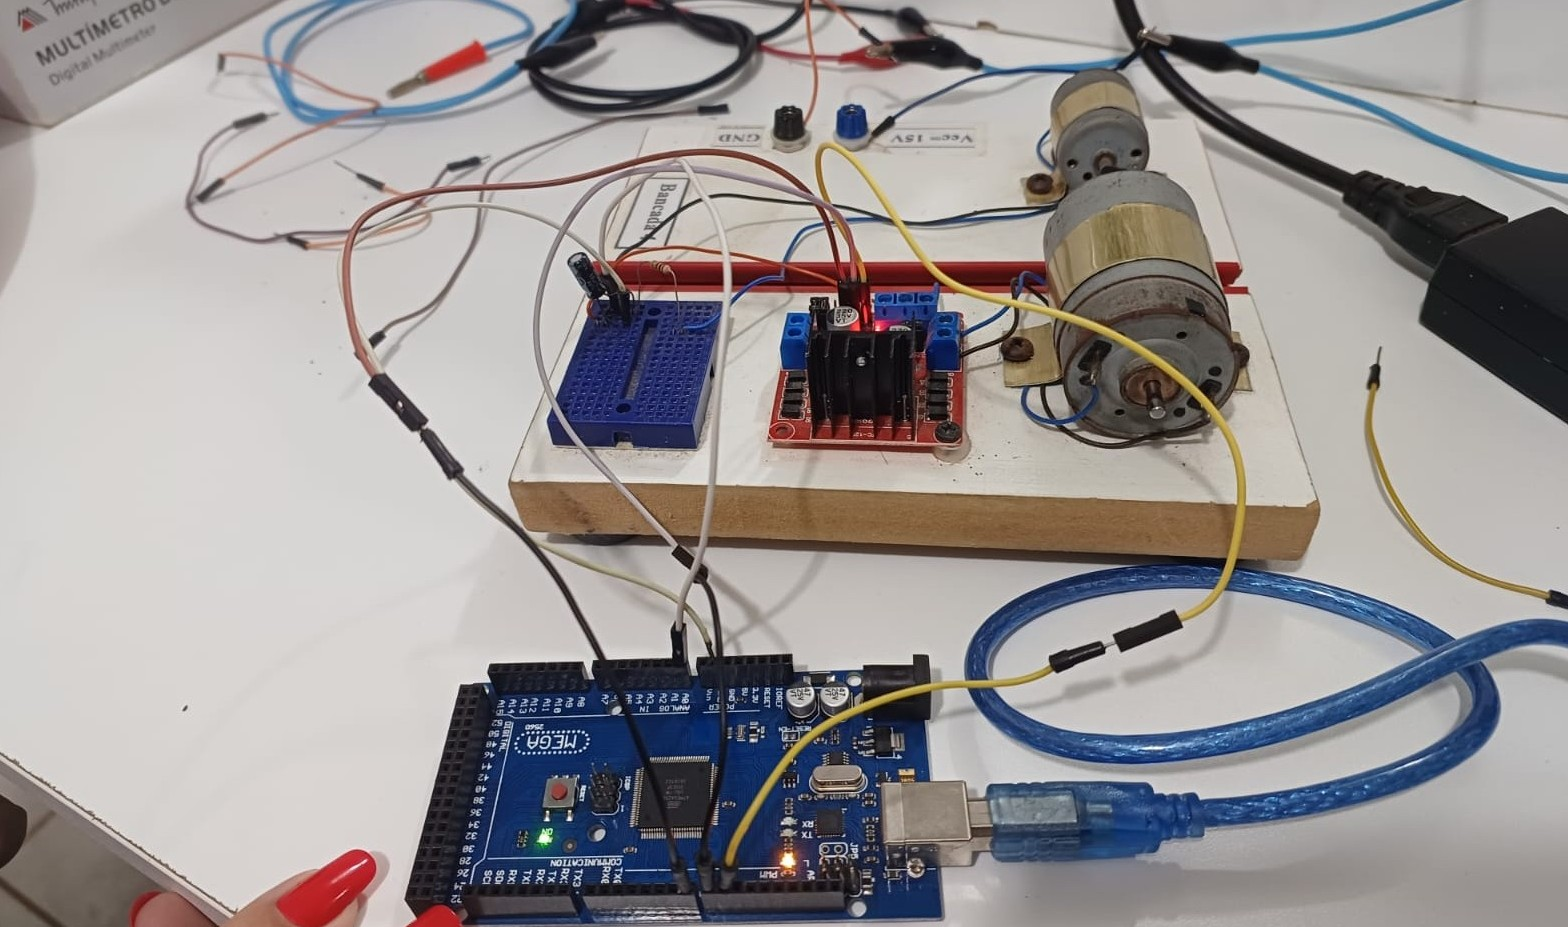
\includegraphics[width=12cm]{../../Figuras/sistema_gerador_motor.jpeg}
		\caption*{Fonte: Autor, (2023)}
	\end{figure}
\end{center}


    \[ G(s) = \frac{K}{\tau s + 1}  \tag{1} \]

\[ y(t) = K A (1 - e^{ - \frac{t}{\tau}}), ~\forall t \geq 0 \tag{2} \]

    \hypertarget{exercuxedcio}{%
\section{Exercício}\label{exercuxedcio}}

\textbf{1. Mostre que para uma entrada degrau de amplitude \(A\) a
resposta do sistema \((1)\) é dada pela equação \((2)\).}

A transformada de Laplace do degrau de amplitude \(A\) é dada pela
equação abaixo,

\[
    \mathcal{L}\{A\} = \dfrac{A}{s}
\]

Com isso, pode-se obter a resposta ao degrau como segue:

\[
    Y(s) = \frac{K}{\tau s + 1} \cdot \frac{A}{s}
\]

A partir da expressão acima, é possível realizar a transformada de
laplace inversa, para isso é preciso decompor o sistema em frações
parciais, como mostrado abaixo:

\[
    \frac{K}{\tau s + 1} \cdot \frac{A}{s} = \frac{KA}{s} - \frac{KA}{\tau s + 1}
\]

Por fim, pode - se aplicar a transformada inversa em ambos os lados:

\[
    \mathcal{L}^{-1}\{Y(s)\} = \mathcal{L}^{-1}\{\frac{KA}{s} - \frac{KA}{\tau s + 1}\}
\]

Assim, o sistema tem resposta no tempo dada por:

\[
    y(t) = KA - KA e^{-\frac{t}{\tau}} = KA(1-e^{-\frac{t}{\tau}})
\]



\textbf{2. Assuma que \(y(\infty) = 3\) para um degrau de \(0.5\) de
amplutude. Determine o o valor do ganho do sistema (\$K =
\textasciitilde{} ? \$).}

Para um sistema de primeira ordem, a resposta ao degrau é dada por:

\[
    y(t)=KA(1-e^{-\frac{t}{\tau}})
\]

Portanto, para um degrau de amplitude \(0.5\), temos:

\[
    y(t) = K(0.5)(1-e^{-\frac{t}{\tau}})
\]

Para \(t \rightarrow \infty\), temos que
\(e^{-\frac{t}{\tau}} \rightarrow 0\). Portanto,
\(y(\infty) = K(0.5) = 3\). Logo, temos:

Quando o tempo \(t\) tende para o infinito, a parcela exponencial da
resposta do sistema tende a zero, com isso, se obtem a expressão abaixo,

\[
    K = \frac{3}{0.5} = 6
\]

Logo, o valor de \(K\) é \$ K=6 \$.



\textbf{3. Para \(K=1,63\) e \(A = 2\). Determine a constante de tempo
do sistema.}

Um sistema de primeira ordem tem que para se obter o valor de \(\tau\)
pode-se usar a seguinteexpressão:

\[
    \tau = \frac{1}{K \cdot A}
\]

Dessa forma, ao substituir os valores dados no enunciado, tem se:

\[
    \tau = \frac{1}{1,63 \cdot 2} \approx 0,306
\]




    \textbf{4. Explique porquê para valores de \(\tau < 0\) o sistema é
instável.}

Para \(\tau < 0\) o Polo do sistema fica no semi-plano direto do plano
complexo, e a teoria de controle nos mostra que para essa configuração
sistema é instável.

    \begin{tcolorbox}[breakable, size=fbox, boxrule=1pt, pad at break*=1mm,colback=cellbackground, colframe=cellborder]
\prompt{In}{incolor}{1}{\boxspacing}
\begin{Verbatim}[commandchars=\\\{\}]
\PY{k+kn}{import} \PY{n+nn}{numpy} \PY{k}{as} \PY{n+nn}{np} 
\PY{k+kn}{import} \PY{n+nn}{matplotlib}\PY{n+nn}{.}\PY{n+nn}{pyplot} \PY{k}{as} \PY{n+nn}{plt}
\PY{k+kn}{import} \PY{n+nn}{pandas} \PY{k}{as} \PY{n+nn}{pd}
\PY{k+kn}{import} \PY{n+nn}{control} \PY{k}{as} \PY{n+nn}{ct}
\PY{k+kn}{import} \PY{n+nn}{scipy}\PY{n+nn}{.}\PY{n+nn}{signal} \PY{k}{as} \PY{n+nn}{sg}
\PY{k+kn}{from} \PY{n+nn}{control}\PY{n+nn}{.}\PY{n+nn}{matlab} \PY{k+kn}{import} \PY{o}{*}

\PY{o}{\PYZpc{}}\PY{k}{config} InlineBackend.figure\PYZus{}format=\PYZsq{}retina\PYZsq{}
\end{Verbatim}
\end{tcolorbox}

    A partir dos dados obtidos será possível encontrar o ganho \(K_m\) e a
constante de tempo \(\tau\).

    \begin{tcolorbox}[breakable, size=fbox, boxrule=1pt, pad at break*=1mm,colback=cellbackground, colframe=cellborder]
\prompt{In}{incolor}{2}{\boxspacing}
\begin{Verbatim}[commandchars=\\\{\}]
\PY{n}{dados} \PY{o}{=} \PY{n}{pd}\PY{o}{.}\PY{n}{read\PYZus{}csv}\PY{p}{(}\PY{l+s+s2}{\PYZdq{}}\PY{l+s+s2}{../dados/piano\PYZus{}Onda\PYZus{}Quadrada\PYZus{}Exemplo.csv}\PY{l+s+s2}{\PYZdq{}}\PY{p}{,} \PY{n}{header} \PY{o}{=} \PY{k+kc}{None}\PY{p}{)}\PY{o}{.}\PY{n}{values}
\PY{n}{dados}
\end{Verbatim}
\end{tcolorbox}

            \begin{tcolorbox}[breakable, size=fbox, boxrule=.5pt, pad at break*=1mm, opacityfill=0]
\prompt{Out}{outcolor}{2}{\boxspacing}
\begin{Verbatim}[commandchars=\\\{\}]
array([[ 0.        ,  0.02      ,  0.04      , {\ldots}, 14.94      ,
        14.96      , 14.98      ],
       [ 8.        ,  8.        ,  8.        , {\ldots},  8.        ,
         8.        ,  8.        ],
       [ 0.        ,  0.        ,  0.        , {\ldots},  2.57      ,
         2.57      ,  2.57      ],
       [ 0.02300167,  0.02000022,  0.020998  , {\ldots},  0.03238726,
         0.03123212,  0.03124857]])
\end{Verbatim}
\end{tcolorbox}
        
    \begin{tcolorbox}[breakable, size=fbox, boxrule=1pt, pad at break*=1mm,colback=cellbackground, colframe=cellborder]
\prompt{In}{incolor}{3}{\boxspacing}
\begin{Verbatim}[commandchars=\\\{\}]
\PY{c+c1}{\PYZsh{} Dados}
\PY{n}{tempo} \PY{o}{=} \PY{n}{dados}\PY{p}{[}\PY{l+m+mi}{0}\PY{p}{,} \PY{p}{:}\PY{p}{]}
\PY{n}{sinal\PYZus{}entrada}  \PY{o}{=} \PY{n}{dados}\PY{p}{[}\PY{l+m+mi}{1}\PY{p}{,} \PY{p}{:}\PY{p}{]}
\PY{n}{sinal\PYZus{}saida} \PY{o}{=} \PY{n}{dados}\PY{p}{[}\PY{l+m+mi}{2}\PY{p}{,} \PY{p}{:}\PY{p}{]}
\PY{n}{toc} \PY{o}{=} \PY{n}{dados}\PY{p}{[}\PY{l+m+mi}{3}\PY{p}{,} \PY{p}{:}\PY{p}{]}

\PY{n}{plt}\PY{o}{.}\PY{n}{figure}\PY{p}{(}\PY{n}{figsize}\PY{o}{=}\PY{p}{(}\PY{l+m+mi}{12}\PY{p}{,} \PY{l+m+mi}{4}\PY{p}{)}\PY{p}{)}
\PY{n}{plt}\PY{o}{.}\PY{n}{plot}\PY{p}{(}\PY{n}{tempo}\PY{p}{,} \PY{n}{sinal\PYZus{}entrada}\PY{p}{,} \PY{n}{c} \PY{o}{=} \PY{l+s+s1}{\PYZsq{}}\PY{l+s+s1}{b}\PY{l+s+s1}{\PYZsq{}}\PY{p}{,} \PY{n}{label} \PY{o}{=} \PY{l+s+s2}{\PYZdq{}}\PY{l+s+s2}{Sinal de Entrada}\PY{l+s+s2}{\PYZdq{}}\PY{p}{)}
\PY{n}{plt}\PY{o}{.}\PY{n}{plot}\PY{p}{(}\PY{n}{tempo}\PY{p}{,} \PY{n}{sinal\PYZus{}saida}\PY{p}{,} \PY{n}{c} \PY{o}{=} \PY{l+s+s1}{\PYZsq{}}\PY{l+s+s1}{r}\PY{l+s+s1}{\PYZsq{}}\PY{p}{,} \PY{n}{label} \PY{o}{=} \PY{l+s+s2}{\PYZdq{}}\PY{l+s+s2}{Sinal de Saída}\PY{l+s+s2}{\PYZdq{}}\PY{p}{)}

\PY{n}{plt}\PY{o}{.} \PY{n}{title}\PY{p}{(}\PY{l+s+s1}{\PYZsq{}}\PY{l+s+s1}{Ensaio Onda Quadrada}\PY{l+s+s1}{\PYZsq{}}\PY{p}{)}
\PY{n}{plt}\PY{o}{.}\PY{n}{ylabel}\PY{p}{(}\PY{l+s+s1}{\PYZsq{}}\PY{l+s+s1}{Tensão (V)}\PY{l+s+s1}{\PYZsq{}}\PY{p}{)}
\PY{n}{plt}\PY{o}{.}\PY{n}{xlabel}\PY{p}{(}\PY{l+s+s1}{\PYZsq{}}\PY{l+s+s1}{tempo (s)}\PY{l+s+s1}{\PYZsq{}}\PY{p}{)}
\PY{n}{plt}\PY{o}{.}\PY{n}{legend}\PY{p}{(}\PY{p}{)}
\PY{n}{plt}\PY{o}{.}\PY{n}{grid}\PY{p}{(}\PY{p}{)}
\PY{n}{plt}\PY{o}{.}\PY{n}{show}\PY{p}{(}\PY{p}{)}

\PY{c+c1}{\PYZsh{} plt.figure()}
\PY{c+c1}{\PYZsh{} plt.plot(tempo,toc)}
\PY{c+c1}{\PYZsh{} plt.show()}

\PY{n}{Ts} \PY{o}{=} \PY{n}{np}\PY{o}{.}\PY{n}{mean}\PY{p}{(}\PY{n}{toc}\PY{p}{)}
\PY{n+nb}{print}\PY{p}{(}\PY{l+s+s1}{\PYZsq{}}\PY{l+s+se}{\PYZbs{}n}\PY{l+s+s1}{\PYZsq{}}\PY{p}{,}\PY{l+s+s1}{\PYZsq{}}\PY{l+s+s1}{Periodo de Amostragem:}\PY{l+s+s1}{\PYZsq{}}\PY{p}{,} \PY{n}{Ts}\PY{p}{)}
\end{Verbatim}
\end{tcolorbox}

    \begin{center}
    \adjustimage{max size={0.9\linewidth}{0.9\paperheight}}{relatorio_sistema_motor_gerador_files/relatorio_sistema_motor_gerador_12_0.png}
    \end{center}
    { \hspace*{\fill} \\}
    
    \begin{Verbatim}[commandchars=\\\{\}]

 Periodo de Amostragem: 0.027902403831481886
    \end{Verbatim}

    \begin{tcolorbox}[breakable, size=fbox, boxrule=1pt, pad at break*=1mm,colback=cellbackground, colframe=cellborder]
\prompt{In}{incolor}{4}{\boxspacing}
\begin{Verbatim}[commandchars=\\\{\}]
\PY{c+c1}{\PYZsh{} Define janela que despreza os primeiros instantes do ensaio}

\PY{n}{janela} \PY{o}{=} \PY{p}{(}\PY{n}{tempo}\PY{o}{\PYZgt{}}\PY{l+m+mi}{2}\PY{p}{)} \PY{o}{\PYZam{}} \PY{p}{(}\PY{n}{tempo}\PY{o}{\PYZlt{}}\PY{l+m+mi}{14}\PY{p}{)}

\PY{c+c1}{\PYZsh{} Obtendo o nível DC da entrada}
\PY{n}{nivel\PYZus{}dc\PYZus{}entrada} \PY{o}{=} \PY{n}{np}\PY{o}{.}\PY{n}{mean}\PY{p}{(}\PY{n}{sinal\PYZus{}entrada}\PY{p}{[}\PY{n}{janela}\PY{p}{]}\PY{p}{)}

\PY{c+c1}{\PYZsh{} Obtendo o nível DC da saída}
\PY{n}{nivel\PYZus{}dc\PYZus{}saida} \PY{o}{=} \PY{n}{np}\PY{o}{.}\PY{n}{mean}\PY{p}{(}\PY{n}{sinal\PYZus{}saida}\PY{p}{[}\PY{n}{janela}\PY{p}{]}\PY{p}{)}

\PY{c+c1}{\PYZsh{} Remove Nivel DC da Entrada e da Saída}
\PY{n}{r} \PY{o}{=} \PY{n}{sinal\PYZus{}entrada} \PY{o}{\PYZhy{}} \PY{n}{nivel\PYZus{}dc\PYZus{}entrada}
\PY{n}{y} \PY{o}{=} \PY{n}{sinal\PYZus{}saida} \PY{o}{\PYZhy{}} \PY{n}{nivel\PYZus{}dc\PYZus{}saida}

\PY{c+c1}{\PYZsh{} Plotagem dos gráficos dos sinais de entrada e saída sem nível DC}
\PY{n}{plt}\PY{o}{.}\PY{n}{figure}\PY{p}{(}\PY{n}{figsize}\PY{o}{=}\PY{p}{(}\PY{l+m+mi}{12}\PY{p}{,} \PY{l+m+mi}{4}\PY{p}{)}\PY{p}{)}
\PY{n}{plt}\PY{o}{.}\PY{n}{plot}\PY{p}{(}\PY{n}{tempo}\PY{p}{[}\PY{n}{janela}\PY{p}{]}\PY{p}{,}\PY{n}{r}\PY{p}{[}\PY{n}{janela}\PY{p}{]}\PY{p}{,} \PY{n}{c} \PY{o}{=} \PY{l+s+s1}{\PYZsq{}}\PY{l+s+s1}{b}\PY{l+s+s1}{\PYZsq{}}\PY{p}{,} \PY{n}{label} \PY{o}{=} \PY{l+s+s2}{\PYZdq{}}\PY{l+s+s2}{Sinal de Entrada}\PY{l+s+s2}{\PYZdq{}}\PY{p}{)}
\PY{n}{plt}\PY{o}{.}\PY{n}{plot}\PY{p}{(}\PY{n}{tempo}\PY{p}{[}\PY{n}{janela}\PY{p}{]}\PY{p}{,}\PY{n}{y}\PY{p}{[}\PY{n}{janela}\PY{p}{]}\PY{p}{,} \PY{n}{c} \PY{o}{=} \PY{l+s+s1}{\PYZsq{}}\PY{l+s+s1}{r}\PY{l+s+s1}{\PYZsq{}}\PY{p}{,} \PY{n}{label} \PY{o}{=} \PY{l+s+s2}{\PYZdq{}}\PY{l+s+s2}{Sinal de Saída}\PY{l+s+s2}{\PYZdq{}}\PY{p}{)}

\PY{n}{plt}\PY{o}{.} \PY{n}{title}\PY{p}{(}\PY{l+s+s1}{\PYZsq{}}\PY{l+s+s1}{Ensaio Onda Quadrada}\PY{l+s+s1}{\PYZsq{}}\PY{p}{)}
\PY{n}{plt}\PY{o}{.}\PY{n}{ylabel}\PY{p}{(}\PY{l+s+s1}{\PYZsq{}}\PY{l+s+s1}{Tensão (V)}\PY{l+s+s1}{\PYZsq{}}\PY{p}{)}
\PY{n}{plt}\PY{o}{.}\PY{n}{xlabel}\PY{p}{(}\PY{l+s+s1}{\PYZsq{}}\PY{l+s+s1}{tempo (s)}\PY{l+s+s1}{\PYZsq{}}\PY{p}{)}
\PY{n}{plt}\PY{o}{.}\PY{n}{legend}\PY{p}{(}\PY{p}{)}
\PY{n}{plt}\PY{o}{.}\PY{n}{grid}\PY{p}{(}\PY{p}{)}
\PY{n}{plt}\PY{o}{.}\PY{n}{show}\PY{p}{(}\PY{p}{)}

\PY{n+nb}{print}\PY{p}{(}\PY{l+s+s2}{\PYZdq{}}\PY{l+s+s2}{Nivel DC entrada:}\PY{l+s+s2}{\PYZdq{}} \PY{p}{,} \PY{n}{nivel\PYZus{}dc\PYZus{}entrada} \PY{p}{)}
\PY{n+nb}{print}\PY{p}{(}\PY{l+s+s2}{\PYZdq{}}\PY{l+s+s2}{Nivel DC saída:}\PY{l+s+s2}{\PYZdq{}} \PY{p}{,} \PY{n}{nivel\PYZus{}dc\PYZus{}saida} \PY{p}{)}
\end{Verbatim}
\end{tcolorbox}

    \begin{center}
    \adjustimage{max size={0.9\linewidth}{0.9\paperheight}}{relatorio_sistema_motor_gerador_files/relatorio_sistema_motor_gerador_13_0.png}
    \end{center}
    { \hspace*{\fill} \\}
    
    \begin{Verbatim}[commandchars=\\\{\}]
Nivel DC entrada: 7.004991680532446
Nivel DC saída: 2.385623960066556
    \end{Verbatim}

    \hypertarget{identificauxe7uxe3o-de-um-modelo-de-primeira-ordem-em-torno-de-um-ponto-de-operauxe7uxe3o}{%
\section{Identificação de um modelo de primeira ordem em torno de um
ponto de
operação}\label{identificauxe7uxe3o-de-um-modelo-de-primeira-ordem-em-torno-de-um-ponto-de-operauxe7uxe3o}}

    \[\boxed{G(s) = \frac{\Delta Y(s)}{\Delta U(s)} = \frac{K}{\tau s + 1}, ~ K = \frac{\delta y}{\delta u}, ~ \tau = t(63 \%) }\]

Para encontrar o ganho \(K_m\) foi feito o calculo para diferentes
intervalos de tempo, com os valores obtidos se obteve a média. o mesmo
procedimento foi realizado para se obter \(\tau\).

    \begin{tcolorbox}[breakable, size=fbox, boxrule=1pt, pad at break*=1mm,colback=cellbackground, colframe=cellborder]
\prompt{In}{incolor}{5}{\boxspacing}
\begin{Verbatim}[commandchars=\\\{\}]
\PY{c+c1}{\PYZsh{} Função para obter os valores de cada variação do sinal de saída}
\PY{k}{def} \PY{n+nf}{calculo\PYZus{}km\PYZus{}tau}\PY{p}{(}\PY{n}{tempo}\PY{p}{,} \PY{n}{y}\PY{p}{,} \PY{n}{inicio}\PY{o}{=}\PY{l+m+mf}{3.9}\PY{p}{,} \PY{n}{fim}\PY{o}{=}\PY{l+m+mf}{5.1}\PY{p}{)}\PY{p}{:}
    \PY{n}{index} \PY{o}{=} \PY{p}{(}\PY{n}{tempo} \PY{o}{\PYZgt{}} \PY{n}{inicio}\PY{p}{)} \PY{o}{\PYZam{}} \PY{p}{(}\PY{n}{tempo} \PY{o}{\PYZlt{}} \PY{n}{fim}\PY{p}{)}
    \PY{n}{t} \PY{o}{=} \PY{n}{tempo}\PY{p}{[}\PY{n}{index}\PY{p}{]}
    \PY{n}{y} \PY{o}{=} \PY{n}{y}\PY{p}{[}\PY{n}{index}\PY{p}{]}
    \PY{n}{ymin} \PY{o}{=} \PY{n}{np}\PY{o}{.}\PY{n}{min}\PY{p}{(}\PY{n}{y}\PY{p}{)}
    \PY{n}{ymax} \PY{o}{=} \PY{n}{np}\PY{o}{.}\PY{n}{max}\PY{p}{(}\PY{n}{y}\PY{p}{)}

    \PY{n}{delta\PYZus{}y} \PY{o}{=} \PY{n+nb}{abs}\PY{p}{(}\PY{n}{ymax} \PY{o}{\PYZhy{}} \PY{n}{ymin}\PY{p}{)}
    \PY{n}{ytau} \PY{o}{=} \PY{p}{(}\PY{l+m+mf}{0.6312}\PY{o}{*}\PY{n}{delta\PYZus{}y}\PY{p}{)} \PY{o}{+} \PY{n}{ymin}

    \PY{k}{return} \PY{p}{[}\PY{n}{t}\PY{p}{,} \PY{n}{y}\PY{p}{]}\PY{p}{,} \PY{p}{[}\PY{n}{ytau}\PY{p}{,} \PY{n}{delta\PYZus{}y}\PY{p}{,} \PY{n}{ymin}\PY{p}{,} \PY{n}{ymax}\PY{p}{]}

\PY{c+c1}{\PYZsh{} Obtendo os intervalos de subida do sinal de saída para plotagens}
\PY{n}{ty1}\PY{p}{,} \PY{n}{ymm1} \PY{o}{=} \PY{n}{calculo\PYZus{}km\PYZus{}tau}\PY{p}{(}\PY{n}{tempo}\PY{p}{,} \PY{n}{y}\PY{p}{,} \PY{n}{inicio}\PY{o}{=}\PY{l+m+mf}{1.9}\PY{p}{,} \PY{n}{fim}\PY{o}{=}\PY{l+m+mf}{3.1}\PY{p}{)}
\PY{n}{km1} \PY{o}{=} \PY{n}{ymm1}\PY{p}{[}\PY{l+m+mi}{1}\PY{p}{]}\PY{o}{/}\PY{l+m+mf}{2.}

\PY{n}{ty2}\PY{p}{,} \PY{n}{ymm2} \PY{o}{=} \PY{n}{calculo\PYZus{}km\PYZus{}tau}\PY{p}{(}\PY{n}{tempo}\PY{p}{,} \PY{n}{y}\PY{p}{,} \PY{n}{inicio}\PY{o}{=}\PY{l+m+mf}{3.9}\PY{p}{,} \PY{n}{fim}\PY{o}{=}\PY{l+m+mf}{5.1}\PY{p}{)}
\PY{n}{km2} \PY{o}{=} \PY{n}{ymm2}\PY{p}{[}\PY{l+m+mi}{1}\PY{p}{]}\PY{o}{/}\PY{l+m+mf}{2.}

\PY{n}{ty3}\PY{p}{,} \PY{n}{ymm3} \PY{o}{=} \PY{n}{calculo\PYZus{}km\PYZus{}tau}\PY{p}{(}\PY{n}{tempo}\PY{p}{,} \PY{n}{y}\PY{p}{,} \PY{n}{inicio}\PY{o}{=}\PY{l+m+mf}{5.9}\PY{p}{,} \PY{n}{fim}\PY{o}{=}\PY{l+m+mf}{7.1}\PY{p}{)}
\PY{n}{km3} \PY{o}{=} \PY{n}{ymm3}\PY{p}{[}\PY{l+m+mi}{1}\PY{p}{]}\PY{o}{/}\PY{l+m+mf}{2.}

\PY{n}{ty4}\PY{p}{,} \PY{n}{ymm4} \PY{o}{=} \PY{n}{calculo\PYZus{}km\PYZus{}tau}\PY{p}{(}\PY{n}{tempo}\PY{p}{,} \PY{n}{y}\PY{p}{,} \PY{n}{inicio}\PY{o}{=}\PY{l+m+mf}{7.9}\PY{p}{,} \PY{n}{fim}\PY{o}{=}\PY{l+m+mf}{9.1}\PY{p}{)}
\PY{n}{km4} \PY{o}{=} \PY{n}{ymm4}\PY{p}{[}\PY{l+m+mi}{1}\PY{p}{]}\PY{o}{/}\PY{l+m+mf}{2.}

\PY{n}{ty5}\PY{p}{,} \PY{n}{ymm5} \PY{o}{=} \PY{n}{calculo\PYZus{}km\PYZus{}tau}\PY{p}{(}\PY{n}{tempo}\PY{p}{,} \PY{n}{y}\PY{p}{,} \PY{n}{inicio}\PY{o}{=}\PY{l+m+mf}{9.9}\PY{p}{,} \PY{n}{fim}\PY{o}{=}\PY{l+m+mf}{11.1}\PY{p}{)}
\PY{n}{km5} \PY{o}{=} \PY{n}{ymm5}\PY{p}{[}\PY{l+m+mi}{1}\PY{p}{]}\PY{o}{/}\PY{l+m+mf}{2.}

\PY{n}{ty6}\PY{p}{,} \PY{n}{ymm6} \PY{o}{=} \PY{n}{calculo\PYZus{}km\PYZus{}tau}\PY{p}{(}\PY{n}{tempo}\PY{p}{,} \PY{n}{y}\PY{p}{,} \PY{n}{inicio}\PY{o}{=}\PY{l+m+mf}{11.9}\PY{p}{,} \PY{n}{fim}\PY{o}{=}\PY{l+m+mf}{13.1}\PY{p}{)}
\PY{n}{km6} \PY{o}{=} \PY{n}{ymm6}\PY{p}{[}\PY{l+m+mi}{1}\PY{p}{]}\PY{o}{/}\PY{l+m+mf}{2.}

\PY{n+nb}{print}\PY{p}{(}\PY{l+s+s2}{\PYZdq{}}\PY{l+s+se}{\PYZbs{}n}\PY{l+s+se}{\PYZbs{}n}\PY{l+s+s2}{Ganho do Sistema}\PY{l+s+s2}{\PYZdq{}}\PY{p}{)}
\PY{n}{kms} \PY{o}{=} \PY{p}{[}\PY{n}{km1}\PY{p}{,} \PY{n}{km2}\PY{p}{,} \PY{n}{km3}\PY{p}{,} \PY{n}{km4}\PY{p}{,} \PY{n}{km5}\PY{p}{,} \PY{n}{km6}\PY{p}{]}
\PY{n+nb}{print}\PY{p}{(}\PY{l+s+sa}{f}\PY{l+s+s2}{\PYZdq{}}\PY{l+s+s2}{Valores de Km : }\PY{l+s+si}{\PYZob{}}\PY{p}{[}\PY{n+nb}{round}\PY{p}{(}\PY{n}{km}\PY{p}{,}\PY{+w}{ }\PY{l+m+mi}{5}\PY{p}{)}\PY{+w}{ }\PY{k}{for}\PY{+w}{ }\PY{n}{km}\PY{+w}{ }\PY{o+ow}{in}\PY{+w}{ }\PY{n}{kms}\PY{p}{]}\PY{l+s+si}{\PYZcb{}}\PY{l+s+s2}{\PYZdq{}}\PY{p}{)}

\PY{n+nb}{print}\PY{p}{(}\PY{l+s+s2}{\PYZdq{}}\PY{l+s+se}{\PYZbs{}n}\PY{l+s+se}{\PYZbs{}n}\PY{l+s+s2}{Constante de Tempo do Sistema}\PY{l+s+se}{\PYZbs{}n}\PY{l+s+s2}{\PYZdq{}}\PY{p}{)}
\PY{n}{taus} \PY{o}{=} \PY{p}{[}\PY{l+m+mf}{0.150}\PY{p}{,} \PY{l+m+mf}{0.155}\PY{p}{,} \PY{l+m+mf}{0.185}\PY{p}{,} \PY{l+m+mf}{0.140}\PY{p}{,} \PY{l+m+mf}{0.155}\PY{p}{,} \PY{l+m+mf}{0.165}\PY{p}{]}
\PY{n+nb}{print}\PY{p}{(}\PY{l+s+sa}{f}\PY{l+s+s2}{\PYZdq{}}\PY{l+s+s2}{Valores de tau : }\PY{l+s+si}{\PYZob{}}\PY{n}{taus}\PY{l+s+si}{\PYZcb{}}\PY{l+s+s2}{\PYZdq{}}\PY{p}{)}

\PY{c+c1}{\PYZsh{} Subgráficos de cada intervalo de subida do sinal de saída}
\PY{n}{fig}\PY{p}{,} \PY{n}{ax} \PY{o}{=} \PY{n}{plt}\PY{o}{.}\PY{n}{subplots}\PY{p}{(}\PY{l+m+mi}{2}\PY{p}{,} \PY{l+m+mi}{3}\PY{p}{,} \PY{n}{figsize}\PY{o}{=}\PY{p}{(}\PY{l+m+mi}{12}\PY{p}{,} \PY{l+m+mi}{5}\PY{p}{)}\PY{p}{)}
\PY{n}{plt}\PY{o}{.}\PY{n}{tight\PYZus{}layout}\PY{p}{(}\PY{p}{)}
\PY{n}{ax}\PY{p}{[}\PY{l+m+mi}{0}\PY{p}{,} \PY{l+m+mi}{0}\PY{p}{]}\PY{o}{.}\PY{n}{plot}\PY{p}{(}\PY{n}{ty1}\PY{p}{[}\PY{l+m+mi}{0}\PY{p}{]}\PY{p}{,} \PY{n}{ty1}\PY{p}{[}\PY{l+m+mi}{1}\PY{p}{]}\PY{p}{,} \PY{l+s+s1}{\PYZsq{}}\PY{l+s+s1}{\PYZhy{}or}\PY{l+s+s1}{\PYZsq{}}\PY{p}{)}
\PY{n}{ax}\PY{p}{[}\PY{l+m+mi}{0}\PY{p}{,} \PY{l+m+mi}{0}\PY{p}{]}\PY{o}{.}\PY{n}{set\PYZus{}yticks}\PY{p}{(}\PY{p}{[}\PY{n}{ymm1}\PY{p}{[}\PY{l+m+mi}{2}\PY{p}{]}\PY{p}{,} \PY{n}{ymm1}\PY{p}{[}\PY{l+m+mi}{0}\PY{p}{]}\PY{p}{,} \PY{n}{ymm1}\PY{p}{[}\PY{l+m+mi}{3}\PY{p}{]}\PY{p}{]}\PY{p}{)}
\PY{n}{ax}\PY{p}{[}\PY{l+m+mi}{0}\PY{p}{,} \PY{l+m+mi}{0}\PY{p}{]}\PY{o}{.}\PY{n}{set\PYZus{}xticks}\PY{p}{(}\PY{p}{[}\PY{l+m+mi}{2}\PY{p}{,} \PY{l+m+mf}{2.150}\PY{p}{]}\PY{p}{)}
\PY{n}{ax}\PY{p}{[}\PY{l+m+mi}{0}\PY{p}{,} \PY{l+m+mi}{0}\PY{p}{]}\PY{o}{.}\PY{n}{grid}\PY{p}{(}\PY{p}{)}


\PY{n}{ax}\PY{p}{[}\PY{l+m+mi}{0}\PY{p}{,} \PY{l+m+mi}{1}\PY{p}{]}\PY{o}{.}\PY{n}{plot}\PY{p}{(}\PY{n}{ty2}\PY{p}{[}\PY{l+m+mi}{0}\PY{p}{]}\PY{p}{,} \PY{n}{ty2}\PY{p}{[}\PY{l+m+mi}{1}\PY{p}{]}\PY{p}{,} \PY{l+s+s1}{\PYZsq{}}\PY{l+s+s1}{\PYZhy{}or}\PY{l+s+s1}{\PYZsq{}}\PY{p}{)}
\PY{n}{ax}\PY{p}{[}\PY{l+m+mi}{0}\PY{p}{,} \PY{l+m+mi}{1}\PY{p}{]}\PY{o}{.}\PY{n}{set\PYZus{}yticks}\PY{p}{(}\PY{p}{[}\PY{n}{ymm2}\PY{p}{[}\PY{l+m+mi}{2}\PY{p}{]}\PY{p}{,} \PY{n}{ymm2}\PY{p}{[}\PY{l+m+mi}{0}\PY{p}{]}\PY{p}{,} \PY{n}{ymm2}\PY{p}{[}\PY{l+m+mi}{3}\PY{p}{]}\PY{p}{]}\PY{p}{)}
\PY{n}{ax}\PY{p}{[}\PY{l+m+mi}{0}\PY{p}{,} \PY{l+m+mi}{1}\PY{p}{]}\PY{o}{.}\PY{n}{set\PYZus{}xticks}\PY{p}{(}\PY{p}{[}\PY{l+m+mi}{4}\PY{p}{,} \PY{l+m+mf}{4.155}\PY{p}{]}\PY{p}{)}
\PY{n}{ax}\PY{p}{[}\PY{l+m+mi}{0}\PY{p}{,} \PY{l+m+mi}{1}\PY{p}{]}\PY{o}{.}\PY{n}{grid}\PY{p}{(}\PY{p}{)}

\PY{n}{ax}\PY{p}{[}\PY{l+m+mi}{0}\PY{p}{,} \PY{l+m+mi}{2}\PY{p}{]}\PY{o}{.}\PY{n}{plot}\PY{p}{(}\PY{n}{ty3}\PY{p}{[}\PY{l+m+mi}{0}\PY{p}{]}\PY{p}{,} \PY{n}{ty3}\PY{p}{[}\PY{l+m+mi}{1}\PY{p}{]}\PY{p}{,} \PY{l+s+s1}{\PYZsq{}}\PY{l+s+s1}{\PYZhy{}or}\PY{l+s+s1}{\PYZsq{}}\PY{p}{)}
\PY{n}{ax}\PY{p}{[}\PY{l+m+mi}{0}\PY{p}{,} \PY{l+m+mi}{2}\PY{p}{]}\PY{o}{.}\PY{n}{set\PYZus{}yticks}\PY{p}{(}\PY{p}{[}\PY{n}{ymm3}\PY{p}{[}\PY{l+m+mi}{2}\PY{p}{]}\PY{p}{,} \PY{n}{ymm3}\PY{p}{[}\PY{l+m+mi}{0}\PY{p}{]}\PY{p}{,} \PY{n}{ymm3}\PY{p}{[}\PY{l+m+mi}{3}\PY{p}{]}\PY{p}{]}\PY{p}{)}
\PY{n}{ax}\PY{p}{[}\PY{l+m+mi}{0}\PY{p}{,} \PY{l+m+mi}{2}\PY{p}{]}\PY{o}{.}\PY{n}{set\PYZus{}xticks}\PY{p}{(}\PY{p}{[}\PY{l+m+mi}{6}\PY{p}{,} \PY{l+m+mf}{6.185}\PY{p}{]}\PY{p}{)}
\PY{n}{ax}\PY{p}{[}\PY{l+m+mi}{0}\PY{p}{,} \PY{l+m+mi}{2}\PY{p}{]}\PY{o}{.}\PY{n}{grid}\PY{p}{(}\PY{p}{)}

\PY{n}{ax}\PY{p}{[}\PY{l+m+mi}{1}\PY{p}{,} \PY{l+m+mi}{0}\PY{p}{]}\PY{o}{.}\PY{n}{plot}\PY{p}{(}\PY{n}{ty4}\PY{p}{[}\PY{l+m+mi}{0}\PY{p}{]}\PY{p}{,} \PY{n}{ty4}\PY{p}{[}\PY{l+m+mi}{1}\PY{p}{]}\PY{p}{,} \PY{l+s+s1}{\PYZsq{}}\PY{l+s+s1}{\PYZhy{}or}\PY{l+s+s1}{\PYZsq{}}\PY{p}{)}
\PY{n}{ax}\PY{p}{[}\PY{l+m+mi}{1}\PY{p}{,} \PY{l+m+mi}{0}\PY{p}{]}\PY{o}{.}\PY{n}{set\PYZus{}yticks}\PY{p}{(}\PY{p}{[}\PY{n}{ymm4}\PY{p}{[}\PY{l+m+mi}{2}\PY{p}{]}\PY{p}{,} \PY{n}{ymm4}\PY{p}{[}\PY{l+m+mi}{0}\PY{p}{]}\PY{p}{,} \PY{n}{ymm4}\PY{p}{[}\PY{l+m+mi}{3}\PY{p}{]}\PY{p}{]}\PY{p}{)}
\PY{n}{ax}\PY{p}{[}\PY{l+m+mi}{1}\PY{p}{,} \PY{l+m+mi}{0}\PY{p}{]}\PY{o}{.}\PY{n}{set\PYZus{}xticks}\PY{p}{(}\PY{p}{[}\PY{l+m+mi}{8}\PY{p}{,} \PY{l+m+mf}{8.140}\PY{p}{]}\PY{p}{)}
\PY{n}{ax}\PY{p}{[}\PY{l+m+mi}{1}\PY{p}{,} \PY{l+m+mi}{0}\PY{p}{]}\PY{o}{.}\PY{n}{grid}\PY{p}{(}\PY{p}{)}

\PY{n}{ax}\PY{p}{[}\PY{l+m+mi}{1}\PY{p}{,} \PY{l+m+mi}{1}\PY{p}{]}\PY{o}{.}\PY{n}{plot}\PY{p}{(}\PY{n}{ty5}\PY{p}{[}\PY{l+m+mi}{0}\PY{p}{]}\PY{p}{,} \PY{n}{ty5}\PY{p}{[}\PY{l+m+mi}{1}\PY{p}{]}\PY{p}{,} \PY{l+s+s1}{\PYZsq{}}\PY{l+s+s1}{\PYZhy{}or}\PY{l+s+s1}{\PYZsq{}}\PY{p}{)}
\PY{n}{ax}\PY{p}{[}\PY{l+m+mi}{1}\PY{p}{,} \PY{l+m+mi}{1}\PY{p}{]}\PY{o}{.}\PY{n}{set\PYZus{}yticks}\PY{p}{(}\PY{p}{[}\PY{n}{ymm5}\PY{p}{[}\PY{l+m+mi}{2}\PY{p}{]}\PY{p}{,} \PY{n}{ymm5}\PY{p}{[}\PY{l+m+mi}{0}\PY{p}{]}\PY{p}{,} \PY{n}{ymm5}\PY{p}{[}\PY{l+m+mi}{3}\PY{p}{]}\PY{p}{]}\PY{p}{)}
\PY{n}{ax}\PY{p}{[}\PY{l+m+mi}{1}\PY{p}{,} \PY{l+m+mi}{1}\PY{p}{]}\PY{o}{.}\PY{n}{set\PYZus{}xticks}\PY{p}{(}\PY{p}{[}\PY{l+m+mi}{10}\PY{p}{,} \PY{l+m+mf}{10.155}\PY{p}{]}\PY{p}{)}
\PY{n}{ax}\PY{p}{[}\PY{l+m+mi}{1}\PY{p}{,} \PY{l+m+mi}{1}\PY{p}{]}\PY{o}{.}\PY{n}{grid}\PY{p}{(}\PY{p}{)}

\PY{n}{ax}\PY{p}{[}\PY{l+m+mi}{1}\PY{p}{,} \PY{l+m+mi}{2}\PY{p}{]}\PY{o}{.}\PY{n}{plot}\PY{p}{(}\PY{n}{ty6}\PY{p}{[}\PY{l+m+mi}{0}\PY{p}{]}\PY{p}{,} \PY{n}{ty6}\PY{p}{[}\PY{l+m+mi}{1}\PY{p}{]}\PY{p}{,} \PY{l+s+s1}{\PYZsq{}}\PY{l+s+s1}{\PYZhy{}or}\PY{l+s+s1}{\PYZsq{}}\PY{p}{)}
\PY{n}{ax}\PY{p}{[}\PY{l+m+mi}{1}\PY{p}{,} \PY{l+m+mi}{2}\PY{p}{]}\PY{o}{.}\PY{n}{set\PYZus{}yticks}\PY{p}{(}\PY{p}{[}\PY{n}{ymm6}\PY{p}{[}\PY{l+m+mi}{2}\PY{p}{]}\PY{p}{,} \PY{n}{ymm6}\PY{p}{[}\PY{l+m+mi}{0}\PY{p}{]}\PY{p}{,} \PY{n}{ymm6}\PY{p}{[}\PY{l+m+mi}{3}\PY{p}{]}\PY{p}{]}\PY{p}{)}
\PY{n}{ax}\PY{p}{[}\PY{l+m+mi}{1}\PY{p}{,} \PY{l+m+mi}{2}\PY{p}{]}\PY{o}{.}\PY{n}{set\PYZus{}xticks}\PY{p}{(}\PY{p}{[}\PY{l+m+mi}{12}\PY{p}{,} \PY{l+m+mf}{12.165}\PY{p}{]}\PY{p}{)}
\PY{n}{ax}\PY{p}{[}\PY{l+m+mi}{1}\PY{p}{,} \PY{l+m+mi}{2}\PY{p}{]}\PY{o}{.}\PY{n}{grid}\PY{p}{(}\PY{p}{)}

\PY{n}{plt}\PY{o}{.}\PY{n}{show}\PY{p}{(}\PY{p}{)}
\end{Verbatim}
\end{tcolorbox}

    \begin{Verbatim}[commandchars=\\\{\}]


Ganho do Sistema
Valores de Km : [0.18, 0.19, 0.19, 0.195, 0.19, 0.185]


Constante de Tempo do Sistema

Valores de tau : [0.15, 0.155, 0.185, 0.14, 0.155, 0.165]
    \end{Verbatim}

    \begin{center}
    \adjustimage{max size={0.9\linewidth}{0.9\paperheight}}{relatorio_sistema_motor_gerador_files/relatorio_sistema_motor_gerador_16_1.png}
    \end{center}
    { \hspace*{\fill} \\}
    
    \begin{tcolorbox}[breakable, size=fbox, boxrule=1pt, pad at break*=1mm,colback=cellbackground, colframe=cellborder]
\prompt{In}{incolor}{6}{\boxspacing}
\begin{Verbatim}[commandchars=\\\{\}]
\PY{c+c1}{\PYZsh{} Função para obter os valores de cada variação do sinal de saída}
\PY{k}{def} \PY{n+nf}{calculo\PYZus{}km\PYZus{}tau1}\PY{p}{(}\PY{n}{tempo}\PY{p}{,} \PY{n}{y}\PY{p}{,} \PY{n}{inicio}\PY{o}{=}\PY{l+m+mf}{2.9}\PY{p}{,} \PY{n}{fim}\PY{o}{=}\PY{l+m+mf}{4.1}\PY{p}{)}\PY{p}{:}
    \PY{n}{index} \PY{o}{=} \PY{p}{(}\PY{n}{tempo} \PY{o}{\PYZgt{}} \PY{n}{inicio}\PY{p}{)} \PY{o}{\PYZam{}} \PY{p}{(}\PY{n}{tempo} \PY{o}{\PYZlt{}} \PY{n}{fim}\PY{p}{)}
    \PY{n}{t} \PY{o}{=} \PY{n}{tempo}\PY{p}{[}\PY{n}{index}\PY{p}{]}
    \PY{n}{y} \PY{o}{=} \PY{n}{y}\PY{p}{[}\PY{n}{index}\PY{p}{]}
    \PY{n}{ymin} \PY{o}{=} \PY{n}{np}\PY{o}{.}\PY{n}{min}\PY{p}{(}\PY{n}{y}\PY{p}{)}
    \PY{n}{ymax} \PY{o}{=} \PY{n}{np}\PY{o}{.}\PY{n}{max}\PY{p}{(}\PY{n}{y}\PY{p}{)}

    \PY{n}{delta\PYZus{}y} \PY{o}{=} \PY{n+nb}{abs}\PY{p}{(}\PY{n}{ymax} \PY{o}{\PYZhy{}} \PY{n}{ymin}\PY{p}{)}
    \PY{n}{ytau} \PY{o}{=} \PY{o}{\PYZhy{}}\PY{p}{(}\PY{p}{(}\PY{l+m+mf}{0.6312}\PY{o}{*}\PY{n}{delta\PYZus{}y}\PY{p}{)} \PY{o}{+} \PY{n}{ymin}\PY{p}{)}

    \PY{k}{return} \PY{p}{[}\PY{n}{t}\PY{p}{,} \PY{n}{y}\PY{p}{]}\PY{p}{,} \PY{p}{[}\PY{n}{ytau}\PY{p}{,} \PY{n}{delta\PYZus{}y}\PY{p}{,} \PY{n}{ymin}\PY{p}{,} \PY{n}{ymax}\PY{p}{]}

\PY{c+c1}{\PYZsh{} Obtendo os intervalos de subida do sinal de saída para plotagens}
\PY{n}{ty\PYZus{}1}\PY{p}{,} \PY{n}{ymm\PYZus{}1} \PY{o}{=} \PY{n}{calculo\PYZus{}km\PYZus{}tau1}\PY{p}{(}\PY{n}{tempo}\PY{p}{,} \PY{n}{y}\PY{p}{,} \PY{n}{inicio}\PY{o}{=}\PY{l+m+mf}{2.9}\PY{p}{,} \PY{n}{fim}\PY{o}{=}\PY{l+m+mf}{4.1}\PY{p}{)}
\PY{n}{km\PYZus{}1} \PY{o}{=} \PY{n}{ymm\PYZus{}1}\PY{p}{[}\PY{l+m+mi}{1}\PY{p}{]}\PY{o}{/}\PY{l+m+mf}{2.}

\PY{n}{ty\PYZus{}2}\PY{p}{,} \PY{n}{ymm\PYZus{}2} \PY{o}{=} \PY{n}{calculo\PYZus{}km\PYZus{}tau1}\PY{p}{(}\PY{n}{tempo}\PY{p}{,} \PY{n}{y}\PY{p}{,} \PY{n}{inicio}\PY{o}{=}\PY{l+m+mf}{4.9}\PY{p}{,} \PY{n}{fim}\PY{o}{=}\PY{l+m+mf}{6.1}\PY{p}{)}
\PY{n}{km\PYZus{}2} \PY{o}{=} \PY{n}{ymm\PYZus{}2}\PY{p}{[}\PY{l+m+mi}{1}\PY{p}{]}\PY{o}{/}\PY{l+m+mf}{2.}

\PY{n}{ty\PYZus{}3}\PY{p}{,} \PY{n}{ymm\PYZus{}3} \PY{o}{=} \PY{n}{calculo\PYZus{}km\PYZus{}tau1}\PY{p}{(}\PY{n}{tempo}\PY{p}{,} \PY{n}{y}\PY{p}{,} \PY{n}{inicio}\PY{o}{=}\PY{l+m+mf}{6.9}\PY{p}{,} \PY{n}{fim}\PY{o}{=}\PY{l+m+mf}{8.1}\PY{p}{)}
\PY{n}{km\PYZus{}3} \PY{o}{=} \PY{n}{ymm\PYZus{}3}\PY{p}{[}\PY{l+m+mi}{1}\PY{p}{]}\PY{o}{/}\PY{l+m+mf}{2.}

\PY{n}{ty\PYZus{}4}\PY{p}{,} \PY{n}{ymm\PYZus{}4} \PY{o}{=} \PY{n}{calculo\PYZus{}km\PYZus{}tau1}\PY{p}{(}\PY{n}{tempo}\PY{p}{,} \PY{n}{y}\PY{p}{,} \PY{n}{inicio}\PY{o}{=}\PY{l+m+mf}{8.9}\PY{p}{,} \PY{n}{fim}\PY{o}{=}\PY{l+m+mf}{10.1}\PY{p}{)}
\PY{n}{km\PYZus{}4} \PY{o}{=} \PY{n}{ymm\PYZus{}4}\PY{p}{[}\PY{l+m+mi}{1}\PY{p}{]}\PY{o}{/}\PY{l+m+mf}{2.}

\PY{n}{ty\PYZus{}5}\PY{p}{,} \PY{n}{ymm\PYZus{}5} \PY{o}{=} \PY{n}{calculo\PYZus{}km\PYZus{}tau1}\PY{p}{(}\PY{n}{tempo}\PY{p}{,} \PY{n}{y}\PY{p}{,} \PY{n}{inicio}\PY{o}{=}\PY{l+m+mf}{10.9}\PY{p}{,} \PY{n}{fim}\PY{o}{=}\PY{l+m+mf}{12.1}\PY{p}{)}
\PY{n}{km\PYZus{}5} \PY{o}{=} \PY{n}{ymm\PYZus{}5}\PY{p}{[}\PY{l+m+mi}{1}\PY{p}{]}\PY{o}{/}\PY{l+m+mf}{2.}

\PY{n}{ty\PYZus{}6}\PY{p}{,} \PY{n}{ymm\PYZus{}6} \PY{o}{=} \PY{n}{calculo\PYZus{}km\PYZus{}tau1}\PY{p}{(}\PY{n}{tempo}\PY{p}{,} \PY{n}{y}\PY{p}{,} \PY{n}{inicio}\PY{o}{=}\PY{l+m+mf}{12.9}\PY{p}{,} \PY{n}{fim}\PY{o}{=}\PY{l+m+mi}{14}\PY{p}{)}
\PY{n}{km\PYZus{}6} \PY{o}{=} \PY{n}{ymm\PYZus{}6}\PY{p}{[}\PY{l+m+mi}{1}\PY{p}{]}\PY{o}{/}\PY{l+m+mf}{2.}

\PY{n+nb}{print}\PY{p}{(}\PY{l+s+s2}{\PYZdq{}}\PY{l+s+se}{\PYZbs{}n}\PY{l+s+se}{\PYZbs{}n}\PY{l+s+s2}{Ganho do Sistema}\PY{l+s+s2}{\PYZdq{}}\PY{p}{)}
\PY{n}{k\PYZus{}ms} \PY{o}{=} \PY{p}{[}\PY{n}{km\PYZus{}1}\PY{p}{,} \PY{n}{km\PYZus{}2}\PY{p}{,} \PY{n}{km\PYZus{}3}\PY{p}{,} \PY{n}{km\PYZus{}4}\PY{p}{,} \PY{n}{km\PYZus{}5}\PY{p}{,} \PY{n}{km\PYZus{}6}\PY{p}{]}
\PY{n+nb}{print}\PY{p}{(}\PY{l+s+sa}{f}\PY{l+s+s2}{\PYZdq{}}\PY{l+s+s2}{Valores de Km : }\PY{l+s+si}{\PYZob{}}\PY{p}{[}\PY{n+nb}{round}\PY{p}{(}\PY{n}{km}\PY{p}{,}\PY{+w}{ }\PY{l+m+mi}{4}\PY{p}{)}\PY{+w}{ }\PY{k}{for}\PY{+w}{ }\PY{n}{km}\PY{+w}{ }\PY{o+ow}{in}\PY{+w}{ }\PY{n}{k\PYZus{}ms}\PY{p}{]}\PY{l+s+si}{\PYZcb{}}\PY{l+s+s2}{\PYZdq{}}\PY{p}{)}

\PY{n+nb}{print}\PY{p}{(}\PY{l+s+s2}{\PYZdq{}}\PY{l+s+se}{\PYZbs{}n}\PY{l+s+se}{\PYZbs{}n}\PY{l+s+s2}{Constante de Tempo do Sistema}\PY{l+s+se}{\PYZbs{}n}\PY{l+s+s2}{\PYZdq{}}\PY{p}{)}
\PY{n}{taus2} \PY{o}{=} \PY{p}{[}\PY{l+m+mf}{0.165}\PY{p}{,} \PY{l+m+mf}{0.165}\PY{p}{,} \PY{l+m+mf}{0.2}\PY{p}{,} \PY{l+m+mf}{0.165}\PY{p}{,} \PY{l+m+mf}{0.165}\PY{p}{,} \PY{l+m+mf}{0.2}\PY{p}{]}
\PY{n+nb}{print}\PY{p}{(}\PY{l+s+sa}{f}\PY{l+s+s2}{\PYZdq{}}\PY{l+s+s2}{Valores de tau : }\PY{l+s+si}{\PYZob{}}\PY{n}{taus2}\PY{l+s+si}{\PYZcb{}}\PY{l+s+s2}{\PYZdq{}}\PY{p}{)}

\PY{c+c1}{\PYZsh{} Subgráficos de cada intervalo de subida do sinal de saída}
\PY{n}{fig}\PY{p}{,} \PY{n}{ax} \PY{o}{=} \PY{n}{plt}\PY{o}{.}\PY{n}{subplots}\PY{p}{(}\PY{l+m+mi}{2}\PY{p}{,} \PY{l+m+mi}{3}\PY{p}{,} \PY{n}{figsize}\PY{o}{=}\PY{p}{(}\PY{l+m+mi}{12}\PY{p}{,} \PY{l+m+mi}{5}\PY{p}{)}\PY{p}{)}
\PY{n}{plt}\PY{o}{.}\PY{n}{tight\PYZus{}layout}\PY{p}{(}\PY{p}{)}
\PY{n}{ax}\PY{p}{[}\PY{l+m+mi}{0}\PY{p}{,} \PY{l+m+mi}{0}\PY{p}{]}\PY{o}{.}\PY{n}{plot}\PY{p}{(}\PY{n}{ty\PYZus{}1}\PY{p}{[}\PY{l+m+mi}{0}\PY{p}{]}\PY{p}{,} \PY{n}{ty\PYZus{}1}\PY{p}{[}\PY{l+m+mi}{1}\PY{p}{]}\PY{p}{,} \PY{l+s+s1}{\PYZsq{}}\PY{l+s+s1}{\PYZhy{}or}\PY{l+s+s1}{\PYZsq{}}\PY{p}{)}
\PY{n}{ax}\PY{p}{[}\PY{l+m+mi}{0}\PY{p}{,} \PY{l+m+mi}{0}\PY{p}{]}\PY{o}{.}\PY{n}{set\PYZus{}yticks}\PY{p}{(}\PY{p}{[}\PY{n}{ymm\PYZus{}1}\PY{p}{[}\PY{l+m+mi}{2}\PY{p}{]}\PY{p}{,} \PY{n}{ymm\PYZus{}1}\PY{p}{[}\PY{l+m+mi}{0}\PY{p}{]}\PY{p}{,} \PY{n}{ymm\PYZus{}1}\PY{p}{[}\PY{l+m+mi}{3}\PY{p}{]}\PY{p}{]}\PY{p}{)}
\PY{n}{ax}\PY{p}{[}\PY{l+m+mi}{0}\PY{p}{,} \PY{l+m+mi}{0}\PY{p}{]}\PY{o}{.}\PY{n}{set\PYZus{}xticks}\PY{p}{(}\PY{p}{[}\PY{l+m+mi}{3}\PY{p}{,} \PY{l+m+mf}{3.165}\PY{p}{]}\PY{p}{)}
\PY{n}{ax}\PY{p}{[}\PY{l+m+mi}{0}\PY{p}{,} \PY{l+m+mi}{0}\PY{p}{]}\PY{o}{.}\PY{n}{grid}\PY{p}{(}\PY{p}{)}

\PY{n}{ax}\PY{p}{[}\PY{l+m+mi}{0}\PY{p}{,} \PY{l+m+mi}{1}\PY{p}{]}\PY{o}{.}\PY{n}{plot}\PY{p}{(}\PY{n}{ty\PYZus{}2}\PY{p}{[}\PY{l+m+mi}{0}\PY{p}{]}\PY{p}{,} \PY{n}{ty\PYZus{}2}\PY{p}{[}\PY{l+m+mi}{1}\PY{p}{]}\PY{p}{,} \PY{l+s+s1}{\PYZsq{}}\PY{l+s+s1}{\PYZhy{}or}\PY{l+s+s1}{\PYZsq{}}\PY{p}{)}
\PY{n}{ax}\PY{p}{[}\PY{l+m+mi}{0}\PY{p}{,} \PY{l+m+mi}{1}\PY{p}{]}\PY{o}{.}\PY{n}{set\PYZus{}yticks}\PY{p}{(}\PY{p}{[}\PY{n}{ymm\PYZus{}2}\PY{p}{[}\PY{l+m+mi}{2}\PY{p}{]}\PY{p}{,} \PY{n}{ymm\PYZus{}2}\PY{p}{[}\PY{l+m+mi}{0}\PY{p}{]}\PY{p}{,} \PY{n}{ymm\PYZus{}2}\PY{p}{[}\PY{l+m+mi}{3}\PY{p}{]}\PY{p}{]}\PY{p}{)}
\PY{n}{ax}\PY{p}{[}\PY{l+m+mi}{0}\PY{p}{,} \PY{l+m+mi}{1}\PY{p}{]}\PY{o}{.}\PY{n}{set\PYZus{}xticks}\PY{p}{(}\PY{p}{[}\PY{l+m+mi}{5}\PY{p}{,} \PY{l+m+mf}{5.165}\PY{p}{]}\PY{p}{)}
\PY{n}{ax}\PY{p}{[}\PY{l+m+mi}{0}\PY{p}{,} \PY{l+m+mi}{1}\PY{p}{]}\PY{o}{.}\PY{n}{grid}\PY{p}{(}\PY{p}{)}

\PY{n}{ax}\PY{p}{[}\PY{l+m+mi}{0}\PY{p}{,} \PY{l+m+mi}{2}\PY{p}{]}\PY{o}{.}\PY{n}{plot}\PY{p}{(}\PY{n}{ty\PYZus{}3}\PY{p}{[}\PY{l+m+mi}{0}\PY{p}{]}\PY{p}{,} \PY{n}{ty\PYZus{}3}\PY{p}{[}\PY{l+m+mi}{1}\PY{p}{]}\PY{p}{,} \PY{l+s+s1}{\PYZsq{}}\PY{l+s+s1}{\PYZhy{}or}\PY{l+s+s1}{\PYZsq{}}\PY{p}{)}
\PY{n}{ax}\PY{p}{[}\PY{l+m+mi}{0}\PY{p}{,} \PY{l+m+mi}{2}\PY{p}{]}\PY{o}{.}\PY{n}{set\PYZus{}yticks}\PY{p}{(}\PY{p}{[}\PY{n}{ymm\PYZus{}3}\PY{p}{[}\PY{l+m+mi}{2}\PY{p}{]}\PY{p}{,} \PY{n}{ymm\PYZus{}3}\PY{p}{[}\PY{l+m+mi}{0}\PY{p}{]}\PY{p}{,} \PY{n}{ymm\PYZus{}3}\PY{p}{[}\PY{l+m+mi}{3}\PY{p}{]}\PY{p}{]}\PY{p}{)}
\PY{n}{ax}\PY{p}{[}\PY{l+m+mi}{0}\PY{p}{,} \PY{l+m+mi}{2}\PY{p}{]}\PY{o}{.}\PY{n}{set\PYZus{}xticks}\PY{p}{(}\PY{p}{[}\PY{l+m+mi}{7}\PY{p}{,} \PY{l+m+mf}{7.2}\PY{p}{]}\PY{p}{)}
\PY{n}{ax}\PY{p}{[}\PY{l+m+mi}{0}\PY{p}{,} \PY{l+m+mi}{2}\PY{p}{]}\PY{o}{.}\PY{n}{grid}\PY{p}{(}\PY{p}{)}

\PY{n}{ax}\PY{p}{[}\PY{l+m+mi}{1}\PY{p}{,} \PY{l+m+mi}{0}\PY{p}{]}\PY{o}{.}\PY{n}{plot}\PY{p}{(}\PY{n}{ty\PYZus{}4}\PY{p}{[}\PY{l+m+mi}{0}\PY{p}{]}\PY{p}{,} \PY{n}{ty\PYZus{}4}\PY{p}{[}\PY{l+m+mi}{1}\PY{p}{]}\PY{p}{,} \PY{l+s+s1}{\PYZsq{}}\PY{l+s+s1}{\PYZhy{}or}\PY{l+s+s1}{\PYZsq{}}\PY{p}{)}
\PY{n}{ax}\PY{p}{[}\PY{l+m+mi}{1}\PY{p}{,} \PY{l+m+mi}{0}\PY{p}{]}\PY{o}{.}\PY{n}{set\PYZus{}yticks}\PY{p}{(}\PY{p}{[}\PY{n}{ymm\PYZus{}4}\PY{p}{[}\PY{l+m+mi}{2}\PY{p}{]}\PY{p}{,} \PY{n}{ymm\PYZus{}4}\PY{p}{[}\PY{l+m+mi}{0}\PY{p}{]}\PY{p}{,} \PY{n}{ymm\PYZus{}4}\PY{p}{[}\PY{l+m+mi}{3}\PY{p}{]}\PY{p}{]}\PY{p}{)}
\PY{n}{ax}\PY{p}{[}\PY{l+m+mi}{1}\PY{p}{,} \PY{l+m+mi}{0}\PY{p}{]}\PY{o}{.}\PY{n}{set\PYZus{}xticks}\PY{p}{(}\PY{p}{[}\PY{l+m+mi}{9}\PY{p}{,} \PY{l+m+mf}{9.165}\PY{p}{]}\PY{p}{)}
\PY{n}{ax}\PY{p}{[}\PY{l+m+mi}{1}\PY{p}{,} \PY{l+m+mi}{0}\PY{p}{]}\PY{o}{.}\PY{n}{grid}\PY{p}{(}\PY{p}{)}

\PY{n}{ax}\PY{p}{[}\PY{l+m+mi}{1}\PY{p}{,} \PY{l+m+mi}{1}\PY{p}{]}\PY{o}{.}\PY{n}{plot}\PY{p}{(}\PY{n}{ty\PYZus{}5}\PY{p}{[}\PY{l+m+mi}{0}\PY{p}{]}\PY{p}{,} \PY{n}{ty\PYZus{}5}\PY{p}{[}\PY{l+m+mi}{1}\PY{p}{]}\PY{p}{,} \PY{l+s+s1}{\PYZsq{}}\PY{l+s+s1}{\PYZhy{}or}\PY{l+s+s1}{\PYZsq{}}\PY{p}{)}
\PY{n}{ax}\PY{p}{[}\PY{l+m+mi}{1}\PY{p}{,} \PY{l+m+mi}{1}\PY{p}{]}\PY{o}{.}\PY{n}{set\PYZus{}yticks}\PY{p}{(}\PY{p}{[}\PY{n}{ymm\PYZus{}5}\PY{p}{[}\PY{l+m+mi}{2}\PY{p}{]}\PY{p}{,} \PY{n}{ymm\PYZus{}5}\PY{p}{[}\PY{l+m+mi}{0}\PY{p}{]}\PY{p}{,} \PY{n}{ymm\PYZus{}5}\PY{p}{[}\PY{l+m+mi}{3}\PY{p}{]}\PY{p}{]}\PY{p}{)}
\PY{n}{ax}\PY{p}{[}\PY{l+m+mi}{1}\PY{p}{,} \PY{l+m+mi}{1}\PY{p}{]}\PY{o}{.}\PY{n}{set\PYZus{}xticks}\PY{p}{(}\PY{p}{[}\PY{l+m+mi}{11}\PY{p}{,} \PY{l+m+mf}{11.165}\PY{p}{]}\PY{p}{)}
\PY{n}{ax}\PY{p}{[}\PY{l+m+mi}{1}\PY{p}{,} \PY{l+m+mi}{1}\PY{p}{]}\PY{o}{.}\PY{n}{grid}\PY{p}{(}\PY{p}{)}

\PY{n}{ax}\PY{p}{[}\PY{l+m+mi}{1}\PY{p}{,} \PY{l+m+mi}{2}\PY{p}{]}\PY{o}{.}\PY{n}{plot}\PY{p}{(}\PY{n}{ty\PYZus{}6}\PY{p}{[}\PY{l+m+mi}{0}\PY{p}{]}\PY{p}{,} \PY{n}{ty\PYZus{}6}\PY{p}{[}\PY{l+m+mi}{1}\PY{p}{]}\PY{p}{,} \PY{l+s+s1}{\PYZsq{}}\PY{l+s+s1}{\PYZhy{}or}\PY{l+s+s1}{\PYZsq{}}\PY{p}{)}
\PY{n}{ax}\PY{p}{[}\PY{l+m+mi}{1}\PY{p}{,} \PY{l+m+mi}{2}\PY{p}{]}\PY{o}{.}\PY{n}{set\PYZus{}yticks}\PY{p}{(}\PY{p}{[}\PY{n}{ymm\PYZus{}6}\PY{p}{[}\PY{l+m+mi}{2}\PY{p}{]}\PY{p}{,} \PY{n}{ymm\PYZus{}6}\PY{p}{[}\PY{l+m+mi}{0}\PY{p}{]}\PY{p}{,} \PY{n}{ymm\PYZus{}6}\PY{p}{[}\PY{l+m+mi}{3}\PY{p}{]}\PY{p}{]}\PY{p}{)}
\PY{n}{ax}\PY{p}{[}\PY{l+m+mi}{1}\PY{p}{,} \PY{l+m+mi}{2}\PY{p}{]}\PY{o}{.}\PY{n}{set\PYZus{}xticks}\PY{p}{(}\PY{p}{[}\PY{l+m+mi}{13}\PY{p}{,} \PY{l+m+mf}{13.2}\PY{p}{]}\PY{p}{)}
\PY{n}{ax}\PY{p}{[}\PY{l+m+mi}{1}\PY{p}{,} \PY{l+m+mi}{2}\PY{p}{]}\PY{o}{.}\PY{n}{grid}\PY{p}{(}\PY{p}{)}

\PY{n}{plt}\PY{o}{.}\PY{n}{show}\PY{p}{(}\PY{p}{)}
\end{Verbatim}
\end{tcolorbox}

    \begin{Verbatim}[commandchars=\\\{\}]


Ganho do Sistema
Valores de Km : [0.19, 0.19, 0.19, 0.185, 0.19, 0.19]


Constante de Tempo do Sistema

Valores de tau : [0.165, 0.165, 0.2, 0.165, 0.165, 0.2]
    \end{Verbatim}

    \begin{center}
    \adjustimage{max size={0.9\linewidth}{0.9\paperheight}}{relatorio_sistema_motor_gerador_files/relatorio_sistema_motor_gerador_17_1.png}
    \end{center}
    { \hspace*{\fill} \\}
    
    \hypertarget{ganho-do-sistema-k_m}{%
\subsection{\texorpdfstring{Ganho do sistema
\(K_m\)}{Ganho do sistema K\_m}}\label{ganho-do-sistema-k_m}}

    \begin{tcolorbox}[breakable, size=fbox, boxrule=1pt, pad at break*=1mm,colback=cellbackground, colframe=cellborder]
\prompt{In}{incolor}{7}{\boxspacing}
\begin{Verbatim}[commandchars=\\\{\}]
\PY{n}{km} \PY{o}{=} \PY{p}{(}\PY{n}{km1} \PY{o}{+} \PY{n}{km2} \PY{o}{+} \PY{n}{km3} \PY{o}{+} \PY{n}{km4} \PY{o}{+} \PY{n}{km5} \PY{o}{+} \PY{n}{km6} \PY{o}{+} \PY{n}{km\PYZus{}1} \PY{o}{+} \PY{n}{km\PYZus{}2} \PY{o}{+} \PY{n}{km\PYZus{}3} \PY{o}{+} \PY{n}{km\PYZus{}4} \PY{o}{+} \PY{n}{km\PYZus{}5} \PY{o}{+} \PY{n}{km\PYZus{}6}\PY{p}{)}\PY{o}{/}\PY{l+m+mf}{12.}
\PY{n+nb}{print}\PY{p}{(}\PY{l+s+sa}{f}\PY{l+s+s2}{\PYZdq{}}\PY{l+s+se}{\PYZbs{}n}\PY{l+s+s2}{Ganho Km: }\PY{l+s+si}{\PYZob{}}\PY{n}{km}\PY{l+s+si}{\PYZcb{}}\PY{l+s+s2}{\PYZdq{}}\PY{p}{)}
\end{Verbatim}
\end{tcolorbox}

    \begin{Verbatim}[commandchars=\\\{\}]

Ganho Km: 0.18874999999999995
    \end{Verbatim}

    \hypertarget{constante-de-tempo-tau}{%
\subsection{\texorpdfstring{Constante de tempo
\(\tau\)}{Constante de tempo \textbackslash{}tau}}\label{constante-de-tempo-tau}}

    \begin{tcolorbox}[breakable, size=fbox, boxrule=1pt, pad at break*=1mm,colback=cellbackground, colframe=cellborder]
\prompt{In}{incolor}{8}{\boxspacing}
\begin{Verbatim}[commandchars=\\\{\}]
\PY{n}{tau} \PY{o}{=} \PY{p}{(}\PY{n}{np}\PY{o}{.}\PY{n}{sum}\PY{p}{(}\PY{n}{taus}\PY{p}{)} \PY{o}{+} \PY{n}{np}\PY{o}{.}\PY{n}{sum}\PY{p}{(}\PY{n}{taus2}\PY{p}{)}\PY{p}{)}\PY{o}{/}\PY{l+m+mf}{12.}
\PY{n+nb}{print}\PY{p}{(}\PY{l+s+sa}{f}\PY{l+s+s2}{\PYZdq{}}\PY{l+s+se}{\PYZbs{}n}\PY{l+s+s2}{Constante de Tempo do sistema: }\PY{l+s+si}{\PYZob{}}\PY{n}{tau}\PY{l+s+si}{\PYZcb{}}\PY{l+s+s2}{\PYZdq{}}\PY{p}{)}
\end{Verbatim}
\end{tcolorbox}

    \begin{Verbatim}[commandchars=\\\{\}]

Constante de Tempo do sistema: 0.1675
    \end{Verbatim}

    \hypertarget{funuxe7uxe3o-de-transferuxeancia-do-modelo-gs}{%
\subsection{\texorpdfstring{Função de Transferência do Modelo
\(G(s)\)}{Função de Transferência do Modelo G(s)}}\label{funuxe7uxe3o-de-transferuxeancia-do-modelo-gs}}

A partir dos valores encontrados para \(K_m\) e \(\tau\) é possível
simular a resposta do modelo para a entrada quadrada, assim é possível
comparar a resposta do modelo com a resposta real do sistema.

    \begin{tcolorbox}[breakable, size=fbox, boxrule=1pt, pad at break*=1mm,colback=cellbackground, colframe=cellborder]
\prompt{In}{incolor}{9}{\boxspacing}
\begin{Verbatim}[commandchars=\\\{\}]
\PY{n}{num} \PY{o}{=} \PY{p}{[}\PY{n}{km}\PY{p}{]}
\PY{n}{den} \PY{o}{=} \PY{p}{[}\PY{n}{tau}\PY{p}{,} \PY{l+m+mi}{1}\PY{p}{]}

\PY{n}{Gs} \PY{o}{=} \PY{n}{ct}\PY{o}{.}\PY{n}{tf}\PY{p}{(}\PY{n}{num}\PY{p}{,} \PY{n}{den}\PY{p}{)}
\PY{n}{tempo1}\PY{p}{,} \PY{n}{saida\PYZus{}modelo} \PY{o}{=} \PY{n}{ct}\PY{o}{.}\PY{n}{forced\PYZus{}response}\PY{p}{(}\PY{n}{Gs}\PY{p}{,} \PY{n}{T}\PY{o}{=}\PY{n}{tempo}\PY{p}{,} \PY{n}{U}\PY{o}{=}\PY{n}{sinal\PYZus{}entrada}\PY{p}{)}


\PY{c+c1}{\PYZsh{} Tirando a média para subtrair o Nível DC do modelo}
\PY{n}{nivel\PYZus{}dc\PYZus{}modelo} \PY{o}{=} \PY{n}{np}\PY{o}{.}\PY{n}{mean}\PY{p}{(}\PY{n}{saida\PYZus{}modelo}\PY{p}{[}\PY{n}{janela}\PY{p}{]}\PY{p}{)}
\PY{n}{saida\PYZus{}sem\PYZus{}dc\PYZus{}modelo} \PY{o}{=} \PY{n}{saida\PYZus{}modelo}\PY{p}{[}\PY{n}{janela}\PY{p}{]} \PY{o}{\PYZhy{}} \PY{n}{nivel\PYZus{}dc\PYZus{}modelo}

\PY{c+c1}{\PYZsh{} Plotagem dos gráficos dos sinais de entrada e saída sem nível DC}
\PY{n}{plt}\PY{o}{.}\PY{n}{figure}\PY{p}{(}\PY{n}{figsize}\PY{o}{=}\PY{p}{(}\PY{l+m+mi}{12}\PY{p}{,} \PY{l+m+mi}{4}\PY{p}{)}\PY{p}{)}
\PY{n}{plt}\PY{o}{.}\PY{n}{plot}\PY{p}{(}\PY{n}{tempo}\PY{p}{[}\PY{n}{janela}\PY{p}{]}\PY{p}{,}\PY{n}{r}\PY{p}{[}\PY{n}{janela}\PY{p}{]}\PY{p}{,} \PY{n}{c} \PY{o}{=} \PY{l+s+s1}{\PYZsq{}}\PY{l+s+s1}{b}\PY{l+s+s1}{\PYZsq{}}\PY{p}{,} \PY{n}{label} \PY{o}{=} \PY{l+s+s2}{\PYZdq{}}\PY{l+s+s2}{Sinal de Entrada}\PY{l+s+s2}{\PYZdq{}}\PY{p}{)}
\PY{n}{plt}\PY{o}{.}\PY{n}{plot}\PY{p}{(}\PY{n}{tempo}\PY{p}{[}\PY{n}{janela}\PY{p}{]}\PY{p}{,} \PY{n}{y}\PY{p}{[}\PY{n}{janela}\PY{p}{]}\PY{p}{,} \PY{l+s+s1}{\PYZsq{}}\PY{l+s+s1}{r}\PY{l+s+s1}{\PYZsq{}}\PY{p}{,} \PY{n}{label} \PY{o}{=} \PY{l+s+s2}{\PYZdq{}}\PY{l+s+s2}{Sinal de saída Bancada}\PY{l+s+s2}{\PYZdq{}}\PY{p}{)}
\PY{n}{plt}\PY{o}{.}\PY{n}{plot}\PY{p}{(}\PY{n}{tempo}\PY{p}{[}\PY{n}{janela}\PY{p}{]}\PY{p}{,} \PY{n}{saida\PYZus{}sem\PYZus{}dc\PYZus{}modelo}\PY{p}{,} \PY{l+s+s1}{\PYZsq{}}\PY{l+s+s1}{k}\PY{l+s+s1}{\PYZsq{}}\PY{p}{,} \PY{n}{label} \PY{o}{=} \PY{l+s+s2}{\PYZdq{}}\PY{l+s+s2}{Sinal de saída do Modelo}\PY{l+s+s2}{\PYZdq{}}\PY{p}{)}

\PY{n}{plt}\PY{o}{.} \PY{n}{title}\PY{p}{(}\PY{l+s+s1}{\PYZsq{}}\PY{l+s+s1}{Ensaio Onda Quadrada}\PY{l+s+s1}{\PYZsq{}}\PY{p}{)}
\PY{n}{plt}\PY{o}{.}\PY{n}{ylabel}\PY{p}{(}\PY{l+s+s1}{\PYZsq{}}\PY{l+s+s1}{Tensão (V)}\PY{l+s+s1}{\PYZsq{}}\PY{p}{)}
\PY{n}{plt}\PY{o}{.}\PY{n}{xlabel}\PY{p}{(}\PY{l+s+s1}{\PYZsq{}}\PY{l+s+s1}{tempo (s)}\PY{l+s+s1}{\PYZsq{}}\PY{p}{)}
\PY{n}{plt}\PY{o}{.}\PY{n}{legend}\PY{p}{(}\PY{p}{)}
\PY{n}{plt}\PY{o}{.}\PY{n}{grid}\PY{p}{(}\PY{p}{)}
\PY{n}{plt}\PY{o}{.}\PY{n}{show}\PY{p}{(}\PY{p}{)}
\end{Verbatim}
\end{tcolorbox}

    \begin{center}
    \adjustimage{max size={0.9\linewidth}{0.9\paperheight}}{relatorio_sistema_motor_gerador_files/relatorio_sistema_motor_gerador_23_0.png}
    \end{center}
    { \hspace*{\fill} \\}
    
    Ao comparar a resposta do sistema real e do modelo encontrada, é
possível concluir que o processo de identificação do sistema foi
realizado corretamente, já que o sinal de saída do modelo se aproxíma do
sistema real, porém, como o sistema real é não linear, se observa que o
modelo encontrado não tem como saída exatamente a resposta desejada.

    \hypertarget{gruxe1fico-do-sinal-de-sauxedda-do-modelo-encontrado-e-do-sistema-real}{%
\paragraph{Gráfico do sinal de saída do modelo encontrado e do sistema
real}\label{gruxe1fico-do-sinal-de-sauxedda-do-modelo-encontrado-e-do-sistema-real}}

    \begin{tcolorbox}[breakable, size=fbox, boxrule=1pt, pad at break*=1mm,colback=cellbackground, colframe=cellborder]
\prompt{In}{incolor}{10}{\boxspacing}
\begin{Verbatim}[commandchars=\\\{\}]
\PY{c+c1}{\PYZsh{} Plotagem dos gráficos dos sinais de entrada e saída sem nível DC}
\PY{n}{plt}\PY{o}{.}\PY{n}{figure}\PY{p}{(}\PY{n}{figsize}\PY{o}{=}\PY{p}{(}\PY{l+m+mi}{12}\PY{p}{,} \PY{l+m+mi}{4}\PY{p}{)}\PY{p}{)}
\PY{n}{plt}\PY{o}{.}\PY{n}{plot}\PY{p}{(}\PY{n}{tempo}\PY{p}{[}\PY{n}{janela}\PY{p}{]}\PY{p}{,} \PY{n}{y}\PY{p}{[}\PY{n}{janela}\PY{p}{]}\PY{p}{,} \PY{l+s+s1}{\PYZsq{}}\PY{l+s+s1}{\PYZhy{}or}\PY{l+s+s1}{\PYZsq{}}\PY{p}{,} \PY{n}{label} \PY{o}{=} \PY{l+s+s2}{\PYZdq{}}\PY{l+s+s2}{Sinal de saída Bancada}\PY{l+s+s2}{\PYZdq{}}\PY{p}{)}
\PY{n}{plt}\PY{o}{.}\PY{n}{plot}\PY{p}{(}\PY{n}{tempo}\PY{p}{[}\PY{n}{janela}\PY{p}{]}\PY{p}{,} \PY{n}{saida\PYZus{}sem\PYZus{}dc\PYZus{}modelo}\PY{p}{,} \PY{l+s+s1}{\PYZsq{}}\PY{l+s+s1}{k}\PY{l+s+s1}{\PYZsq{}}\PY{p}{,} \PY{n}{label} \PY{o}{=} \PY{l+s+s2}{\PYZdq{}}\PY{l+s+s2}{Sinal de saída do Modelo}\PY{l+s+s2}{\PYZdq{}}\PY{p}{)}

\PY{n}{plt}\PY{o}{.} \PY{n}{title}\PY{p}{(}\PY{l+s+s1}{\PYZsq{}}\PY{l+s+s1}{Ensaio Onda Quadrada}\PY{l+s+s1}{\PYZsq{}}\PY{p}{)}
\PY{n}{plt}\PY{o}{.}\PY{n}{ylabel}\PY{p}{(}\PY{l+s+s1}{\PYZsq{}}\PY{l+s+s1}{Tensão (V)}\PY{l+s+s1}{\PYZsq{}}\PY{p}{)}
\PY{n}{plt}\PY{o}{.}\PY{n}{xlabel}\PY{p}{(}\PY{l+s+s1}{\PYZsq{}}\PY{l+s+s1}{tempo (s)}\PY{l+s+s1}{\PYZsq{}}\PY{p}{)}
\PY{n}{plt}\PY{o}{.}\PY{n}{legend}\PY{p}{(}\PY{p}{)}
\PY{n}{plt}\PY{o}{.}\PY{n}{grid}\PY{p}{(}\PY{p}{)}
\PY{n}{plt}\PY{o}{.}\PY{n}{show}\PY{p}{(}\PY{p}{)}
\end{Verbatim}
\end{tcolorbox}

    \begin{center}
    \adjustimage{max size={0.9\linewidth}{0.9\paperheight}}{relatorio_sistema_motor_gerador_files/relatorio_sistema_motor_gerador_26_0.png}
    \end{center}
    { \hspace*{\fill} \\}
    
    \begin{tcolorbox}[breakable, size=fbox, boxrule=1pt, pad at break*=1mm,colback=cellbackground, colframe=cellborder]
\prompt{In}{incolor}{11}{\boxspacing}
\begin{Verbatim}[commandchars=\\\{\}]
\PY{c+c1}{\PYZsh{} Plotagem dos gráficos dos sinais de entrada e saída sem nível DC}
\PY{n}{plt}\PY{o}{.}\PY{n}{figure}\PY{p}{(}\PY{n}{figsize}\PY{o}{=}\PY{p}{(}\PY{l+m+mi}{12}\PY{p}{,} \PY{l+m+mi}{4}\PY{p}{)}\PY{p}{)}
\PY{n}{plt}\PY{o}{.}\PY{n}{plot}\PY{p}{(}\PY{n}{tempo}\PY{p}{[}\PY{n}{janela}\PY{p}{]}\PY{p}{[}\PY{l+m+mi}{200}\PY{p}{:}\PY{l+m+mi}{400}\PY{p}{]}\PY{p}{,} \PY{n}{y}\PY{p}{[}\PY{n}{janela}\PY{p}{]}\PY{p}{[}\PY{l+m+mi}{200}\PY{p}{:}\PY{l+m+mi}{400}\PY{p}{]}\PY{p}{,} \PY{l+s+s1}{\PYZsq{}}\PY{l+s+s1}{\PYZhy{}or}\PY{l+s+s1}{\PYZsq{}}\PY{p}{,} \PY{n}{label} \PY{o}{=} \PY{l+s+s2}{\PYZdq{}}\PY{l+s+s2}{Sinal de saída Bancada}\PY{l+s+s2}{\PYZdq{}}\PY{p}{)}
\PY{n}{plt}\PY{o}{.}\PY{n}{plot}\PY{p}{(}\PY{n}{tempo}\PY{p}{[}\PY{n}{janela}\PY{p}{]}\PY{p}{[}\PY{l+m+mi}{200}\PY{p}{:}\PY{l+m+mi}{400}\PY{p}{]}\PY{p}{,} \PY{n}{saida\PYZus{}sem\PYZus{}dc\PYZus{}modelo}\PY{p}{[}\PY{l+m+mi}{200}\PY{p}{:}\PY{l+m+mi}{400}\PY{p}{]}\PY{p}{,} \PY{l+s+s1}{\PYZsq{}}\PY{l+s+s1}{k}\PY{l+s+s1}{\PYZsq{}}\PY{p}{,} \PY{n}{label} \PY{o}{=} \PY{l+s+s2}{\PYZdq{}}\PY{l+s+s2}{Sinal de saída do Modelo}\PY{l+s+s2}{\PYZdq{}}\PY{p}{)}

\PY{n}{plt}\PY{o}{.} \PY{n}{title}\PY{p}{(}\PY{l+s+s1}{\PYZsq{}}\PY{l+s+s1}{Ensaio Onda Quadrada}\PY{l+s+s1}{\PYZsq{}}\PY{p}{)}
\PY{n}{plt}\PY{o}{.}\PY{n}{ylabel}\PY{p}{(}\PY{l+s+s1}{\PYZsq{}}\PY{l+s+s1}{Tensão (V)}\PY{l+s+s1}{\PYZsq{}}\PY{p}{)}
\PY{n}{plt}\PY{o}{.}\PY{n}{xlabel}\PY{p}{(}\PY{l+s+s1}{\PYZsq{}}\PY{l+s+s1}{tempo (s)}\PY{l+s+s1}{\PYZsq{}}\PY{p}{)}
\PY{n}{plt}\PY{o}{.}\PY{n}{legend}\PY{p}{(}\PY{p}{)}
\PY{n}{plt}\PY{o}{.}\PY{n}{grid}\PY{p}{(}\PY{p}{)}
\PY{n}{plt}\PY{o}{.}\PY{n}{show}\PY{p}{(}\PY{p}{)}
\end{Verbatim}
\end{tcolorbox}

    \begin{center}
    \adjustimage{max size={0.9\linewidth}{0.9\paperheight}}{relatorio_sistema_motor_gerador_files/relatorio_sistema_motor_gerador_27_0.png}
    \end{center}
    { \hspace*{\fill} \\}
    
    \hypertarget{conclusuxe3o}{%
\section{Conclusão}\label{conclusuxe3o}}

    A identificação de sistemas, portanto, é uma excelente maneira de
encontrar uma aproximação do comportamento do sistema real para um
determinado ponto de operação, no entanto, desse ter em mente que para
cada ponto de operação será necessário encontrar um modelo especifico.


    % Add a bibliography block to the postdoc
    
    
    
\end{document}
